%%% SETUP %%%%%%%%%%%%%%%%%%%%%%%%%%%%%%%%%%%%%%%%%%%%%%%%%%%%%%%%%%%%%%%%%%%%%%

%%% DOCUMENT TYPE %%%%%%%%%%%%%%%%%%%%%%%%%%%%%%%%%%%%%%%%%%%%%%%%%%%%%%%%%%%%%%

\documentclass[10pt,twocolumn, a4paper]{article}

%%% PACKAGES %%%%%%%%%%%%%%%%%%%%%%%%%%%%%%%%%%%%%%%%%%%%%%%%%%%%%%%%%%%%%%%%%%%

% Encoding

\usepackage[utf8]{inputenc}
\usepackage[T1]{fontenc}

% Geometry
\usepackage{multirow}
\usepackage{graphicx}
\usepackage{geometry} % edit margins of paper
\usepackage{setspace} % edit line spacing
\usepackage{fancyhdr} % header, footer
\usepackage{titlesec} % edit format of titles

% Visual

\usepackage[dvipsnames]{xcolor} % colors
\usepackage{tikz} % graphics
\usepackage[framemethod=tikz]{mdframed} % frames, better theorems

% Math

\usepackage{amsmath} % math tools
\usepackage{amssymb} % math symbols
\usepackage{amsthm} % thereoms
\usepackage{mathtools} % math tools

% Referencing

\usepackage{nameref}
\usepackage{hyperref}
\usepackage{cleveref}
% Useful

\usepackage[shortlabels]{enumitem} % enumerations

% Other

\usepackage{lastpage} % get number of last page

%%% MARGINS %%%%%%%%%%%%%%%%%%%%%%%%%%%%%%%%%%%%%%%%%%%%%%%%%%%%%%%%%%%%%%%%%%%%

\geometry{a4paper, left=20mm, right=20mm, top=20mm, bottom=20mm, includehead}

%%% COLORS %%%%%%%%%%%%%%%%%%%%%%%%%%%%%%%%%%%%%%%%%%%%%%%%%%%%%%%%%%%%%%%%%%%%%

%%% TITLES %%%%%%%%%%%%%%%%%%%%%%%%%%%%%%%%%%%%%%%%%%%%%%%%%%%%%%%%%%%%%%%%%%%%%

\colorlet{color-section}                {BrickRed}
\colorlet{color-subsection}             {BrickRed}

%%% MATH BOXES %%%%%%%%%%%%%%%%%%%%%%%%%%%%%%%%%%%%%%%%%%%%%%%%%%%%%%%%%%%%%%%%%

\colorlet{color-definition}             {SpringGreen!20}
\colorlet{color-theorem}                {Apricot!13}
\colorlet{color-proposition}            {Apricot!13}
\colorlet{color-corollary}              {Apricot!13}
\colorlet{color-lemma}                  {Apricot!13}
\colorlet{color-remark}                 {Gray!5}
\colorlet{color-example}                {Lavender!7}
% \colorlet{color-proof}                  {FILL COLOR HERE}


%%% CAPTIONS %%%%%%%%%%%%%%%%%%%%%%%%%%%%%%%%%%%%%%%%%%%%%%%%%%%%%%%%%%%%%%%%%%%

%%% CAPTION DEFINITION %%%%%%%%%%%%%%%%%%%%%%%%%%%%%%%%%%%%%%%%%%%%%%%%%%%%%%%%%

\newcommand*{\definitionname}{Definition}
\newcommand*{\theoremname}{Theorem}
\newcommand*{\propositionname}{Proposition}
\newcommand*{\corollaryname}{Corollary}
\newcommand*{\lemmaname}{Lemma}
\newcommand*{\remarkname}{Remark}
\newcommand*{\examplename}{Example}


%%% SHORTCUTS %%%%%%%%%%%%%%%%%%%%%%%%%%%%%%%%%%%%%%%%%%%%%%%%%%%%%%%%%%%%%%%%%%

%%% SINGLE SYMBOLS %%%%%%%%%%%%%%%%%%%%%%%%%%%%%%%%%%%%%%%%%%%%%%%%%%%%%%%%%%%%

% Logic

% \forall exists
% \exists exists
% \lnot exists
% \lor exists
% \land exists
\newcommand*{\limp}{\rightarrow}
\newcommand*{\limps}{\; \limp \;} % \limp with some space around
\newcommand*{\leqv}{\leftrightarrow}
\newcommand*{\leqvs}{\; \leqvs \;} % \leqv with some space around

% Meta Logic

% \implies exists
% \iff exists

% Colon Stuff

\newcommand*{\cl}{\colon}
\newcommand*{\cleq}{\coloneqq}
\newcommand*{\eqcl}{\eqqcolon}

% Sets

\newcommand*{\N}{\mathbb{N}} % natural numbers
\newcommand*{\Z}{\mathbb{Z}} % integers
\newcommand*{\Q}{\mathbb{Q}} % rational numbers
\newcommand*{\R}{\mathbb{R}} % real numbers
\newcommand*{\C}{\mathbb{C}} % complex numbers

%%% MATH OPERATORS %%%%%%%%%%%%%%%%%%%%%%%%%%%%%%%%%%%%%%%%%%%%%%%%%%%%%%%%%%%%%

% General

\DeclareMathOperator{\id}{id}
\DeclareMathOperator{\sgn}{sgn}

%%% TEMPLATES %%%%%%%%%%%%%%%%%%%%%%%%%%%%%%%%%%%%%%%%%%%%%%%%%%%%%%%%%%%%%%%%%%

% General

% write a set definition like: { #1 | #2 }
\newcommand*{\setdefinition}[2]{
  \left\{ #1 \mathrel{}\middle|\mathrel{} #2 \right\}
}

% write a nice map definition
\newcommand*{\mapdefinition}[5]{
  \begin{align*}
    #1 \cl #2 &\to     #3 \\
           #4 &\mapsto #5
  \end{align*}
}


%%% FORMATTING %%%%%%%%%%%%%%%%%%%%%%%%%%%%%%%%%%%%%%%%%%%%%%%%%%%%%%%%%%%%%%%%%

%%% HEADER, FOOTER %%%%%%%%%%%%%%%%%%%%%%%%%%%%%%%%%%%%%%%%%%%%%%%%%%%%%%%%%%%%%

\pagestyle{fancy}
\fancyhf{} % clear everything
\lhead{\sffamily}
\chead{\sffamily \large \bfseries Tichu strategies depending on course of play}
\rhead{\sffamily Page \thepage /\pageref*{LastPage}}
\lfoot{}
\cfoot{}
\rfoot{}

%%% TITLE FORMAT %%%%%%%%%%%%%%%%%%%%%%%%%%%%%%%%%%%%%%%%%%%%%%%%%%%%%%%%%%%%%%%

\setcounter{secnumdepth}{2}

\titleformat{\chapter}[display]
{\normalfont\huge\bfseries}{\chaptertitlename\ \thechapter}{20pt}{\Huge}
\titleformat{\section}[frame]
{\normalfont\LARGE\bfseries\color{color-section}\scshape}{\filright\,\thesection\,}{0.2ex}{\filcenter}
\titleformat{\subsection}
{\normalfont\Large\bfseries\color{color-subsection}}{\thesubsection}{1em}{}
\titleformat{\subsubsection}
{\normalfont\normalsize\bfseries}{\thesubsubsection}{1em}{}
\titleformat{\paragraph}[runin]
{\normalfont\normalsize\bfseries}{\theparagraph}{1em}{}
\titleformat{\subparagraph}[runin]
{\normalfont\normalsize\bfseries}{\thesubparagraph}{1em}{}

%%% SPACING %%%%%%%%%%%%%%%%%%%%%%%%%%%%%%%%%%%%%%%%%%%%%%%%%%%%%%%%%%%%%%

% Titles

\titlespacing*{\chapter}{0pt}{50pt}{40pt}
\titlespacing*{\section}{0pt}{3.5ex plus 1ex minus .2ex}{2.3ex plus .2ex}
\titlespacing*{\subsection}{0pt}{3.25ex plus 1ex minus .2ex}{1.5ex plus .2ex}
\titlespacing*{\subsubsection}{0pt}{3.25ex plus 1ex minus .2ex}{1.5ex plus .2ex}
\titlespacing*{\paragraph}{0pt}{3.25ex plus 1ex minus .2ex}{1em}
\titlespacing*{\subparagraph}{\parindent}{3.25ex plus 1ex minus .2ex}{1em}

% Text, Paragraphs

%\setstretch{1.05} % scaling of space between lines
\setlength{\parindent}{0pt} % indentation of paragraphs
%\setlength{\parskip}{4.0pt plus 1.0pt minus 1.0pt} % space between paragraphs
\setlength{\parskip}{0.8ex}
\setlength{\topsep}{0pt}

%%% SYMBOLS USED BY NUMBERINGS, ENVIRONMENTS, ... %%%%%%%%%%%%%%%%%%%%%%%%%%%%%%

% \renewcommand*\qedsymbol{$\blacksquare$} % alternative QED symbol
\renewcommand{\thefootnote}{\arabic{footnote}} % normal footnotes on page
\renewcommand{\thempfootnote}{\fnsymbol{mpfootnote}} % footnotes on minipages, e.g. in mdframed environments

%%% LISTS, ENUMERATIONS %%%%%%%%%%%%%%%%%%%%%%%%%%%%%%%%%%%%%%%%%%%%%%%%%%%%%%%%

% 'itemize'

\setlist[itemize]{noitemsep, topsep=0pt}

% 'enumerate'

% no special settings at the moment

% 'description'

% no special settings at the moment

% 'axioms'

\newlist{axioms}{enumerate}{2}
\setlist[axioms]{itemsep=0pt,label*=\arabic*.}

%%% MDFRAMED PATCH %%%%%%%%%%%%%%%%%%%%%%%%%%%%%%%%%%%%%%%%%%%%%%%%%%%%%%%%%%%%%

\usepackage{xpatch}

\makeatletter
\xpatchcmd{\endmdframed}
  {\aftergroup\endmdf@trivlist\color@endgroup}
  {\endmdf@trivlist\color@endgroup\@doendpe}
  {}{}
\makeatother

%%% MDFRAMED STYLES %%%%%%%%%%%%%%%%%%%%%%%%%%%%%%%%%%%%%%%%%%%%%%%%%%%%%%%%%%%%

% thick frame and bar for title

\mdfdefinestyle{style-box}{
  skipabove=1.5ex plus .5ex minus .2ex,
  skipbelow=1ex plus .2ex minus .2ex,
  linewidth=2pt,
  linecolor=Gray!20,
%   roundcorner=3pt,
  innerleftmargin=0.5\baselineskip,
  innerrightmargin=0.5\baselineskip,
  innertopmargin=0.4\baselineskip,
  innerbottommargin=0.4\baselineskip,
  frametitlebackgroundcolor=Gray!20,
  frametitleaboveskip=0.3pt,
  frametitlebelowskip=0.3pt,
  theoremseparator=,
  theoremspace=\hfill,
  theoremtitlefont=\mdseries\scshape,
  nobreak=true
}

% highlighted background

\mdfdefinestyle{style-background}{
  skipabove=1.5ex plus .5ex minus .2ex,
  skipbelow=1ex plus .2ex minus .2ex,
  hidealllines=true,
  backgroundcolor=Gray!5,
  innerleftmargin=0.5\baselineskip,
  innerrightmargin=0.5\baselineskip,
  innertopmargin=0.4\baselineskip,
  innerbottommargin=0.4\baselineskip,
}

% thin frame

\mdfdefinestyle{style-leftline}{
  skipabove=1.5ex plus .5ex minus .2ex,
  skipbelow=1ex plus .2ex minus .2ex,
  linewidth=1pt,
  linecolor=Gray!50,
  topline=false,
  bottomline=false,
  rightline=false,
  innerleftmargin=0.5\baselineskip,
  innerrightmargin=0,
  innertopmargin=0.2\baselineskip,
  innerbottommargin=0.0\baselineskip,
}

%%% ENVIRONMENTS %%%%%%%%%%%%%%%%%%%%%%%%%%%%%%%%%%%%%%%%%%%%%%%%%%%%%%%%%%%%%%%

% Definition

\mdtheorem[
  style=style-box,
  linecolor=color-definition,
  frametitlebackgroundcolor=color-definition
]{definition}{\definitionname}[section]

% Theorem

\mdtheorem[
  style=style-box,
  linecolor=color-theorem,
  frametitlebackgroundcolor=color-theorem,
  font=\itshape
]{theorem}{\theoremname}[section]

% Proposition

\mdtheorem[
  style=style-box,
  linecolor=color-proposition,
  frametitlebackgroundcolor=color-proposition,
  font=\itshape
]{proposition}[theorem]{\propositionname}

% Corollary

\mdtheorem[
  style=style-box,
  linecolor=color-corollary,
  frametitlebackgroundcolor=color-corollary,
  font=\itshape
]{corollary}[theorem]{\corollaryname}

% Lemma

\mdtheorem[
  style=style-box,
  linecolor=color-lemma,
  frametitlebackgroundcolor=color-lemma,
  font=\itshape
]{lemma}[theorem]{\lemmaname}

\theoremstyle{remark}

% Remark

\newtheorem*{remark}{\remarkname}
\surroundwithmdframed[
  style=style-background,
  backgroundcolor=color-remark
]{remark}

% Example

\newtheorem*{example}{\examplename}
\surroundwithmdframed[
  style=style-background,
  backgroundcolor=color-example
]{example}

% Proof

\surroundwithmdframed[
  style=style-leftline
]{proof}

%%% TEXT FORMATTING %%%%%%%%%%%%%%%%%%%%%%%%%%%%%%%%%%%%%%%%%%%%%%%%%%%%%%%%%%%%

% definitions

\newcommand*{\df}[1]{\textbf{#1}}



%%% LANGUAGE %%%%%%%%%%%%%%%%%%%%%%%%%%%%%%%%%%%%%%%%%%%%%%%%%%%%%%%%%%%%%%%%%%%

%%% SETUP %%%%%%%%%%%%%%%%%%%%%%%%%%%%%%%%%%%%%%%%%%%%%%%%%%%%%%%%%%%%%%%%%%%%%%

\usepackage[english]{babel}

%%% CAPTION REDEFINITION %%%%%%%%%%%%%%%%%%%%%%%%%%%%%%%%%%%%%%%%%%%%%%%%%%%%%%%



%%% HYPHENATION %%%%%%%%%%%%%%%%%%%%%%%%%%%%%%%%%%%%%%%%%%%%%%%%%%%%%%%%%%%%%%%%




%%% DOCUMENT %%%%%%%%%%%%%%%%%%%%%%%%%%%%%%%%%%%%%%%%%%%%%%%%%%%%%%%%%%%%%%%%%%%
%\usepackage{slashbox}
\usepackage{multirow}
\usepackage{listings}
\usepackage{commath}
\usepackage{subcaption}
\usepackage{float}

\begin{document}

\title{Tichu strategies depending on course of play}
\date{June 03, 2020}
\author{Matthias Schmickler \and Paul Sander \and Jean-Luc Portner \and Tom Haidinger \and Andrey Bryutkin \\ \\ Swiss Federal Institute of Technology Zurich (ETH)}
\maketitle

\section*{Abstract}
We shall start with an introduction to the game along with an optional explanation section for readers not experienced with the game of Tichu. This is followed by basic assumptions and approximations we reach in order to dissect the game-theoretical mechanisms into distinct entities that we model throughout this essay. After a thorough analysis of our theoretical models, including discussions concerning their logical semantics, we implement real world data into our models. These implemented variables derive from a dataset of more than 10,000 datapoints collected from onlinetichu.com using a webscrapper and a short survey we distributed. We then draw some conclusions by inspecting the nash equilibrium for one specifc game mechansim. Finally, we simulate 10,000s of games through our own programms and manipulate multiple variables to draw conclusions regarding stragety and responses to specific circumstances, requiring over 50 hours of computing with the help of ETH‘s Euler computer. Lastly, we evaluate aspects of our results and suggest improvments and identify weaknesses in our approximations to hopefully cumulate into concrete advice for this game.

\section{Motivation and goals}

A prevalent characteristic of both mathematics and physics is their elaborate structure of interdependent concepts. It is only natural, then, for us students to thrive off of complexity and intricateness both within our courses as well as throughout our daily life. One such endeavour we satisfy our free time with is the game of Tichu. Tichu is a team card game taught to us by older students of our courses during the, albeit not very wide-ranging, cultural melting-pot between years – that unproductive period when our courses’ study hall slowly turns into the Mensa. 

    In addition to luck and strategy, this game became popular within our friend-group due to its fairly unique aspect of interaction. Allowing for multiple possible card combinations, special cards and a process of card switching, Tichu derives its complexity not through complicated rules, but rather through diverseness of strategy. Indeed, given one must adapt to one’s opponents’ and teammate’s strategies, one may say its strategies are interactive and reactive in nature. Therefore – although we note that card games are hard to analyse in general – we believe Tichu is indeed approachable through game-theoretic methods. 

    Fascinated by this type of game and equipped with tools from our game theory course, we pose the general question: “which strategy should we pursue as players?”. We shall further differentiate this admittedly vague question into: “what strategy should we pursue given”: a) “we know what player-type all other players are” and b) “we do not know anything about other players”. 
\section{Introduction on Tichu}

Tichu is a complicated team card game with many rounds that will be explained in detail below. The gist of it is that a set of playing cards is distributed among four players, two of which form a team, and card combinations are played to trump each other and win cards that score different amounts of points. At the beginning of each round each player exchanges a card with every other player, influencing the player dynamics of each round. Additionally, a bet, called a Tichu, can be placed on exiting a round of the game first, which yields bonus points. Teams then fight to reach 1000 points first. Obviously, this is not a full explanation, rather it serves to highlight the most important aspects of the game and subsequently the most interesting mechanisms explored in this essay, namely: the exchange stage, the player dynamics and the betting mechanism of a Tichu. 

A game of Tichu consists of two teams with two players each. The game is divided into multiple rounds that host opportunities to score and even lose points. The game ends when one team has collected 1000 or more points. In every round of the game each player is dealt 14 cards from the 56-card deck. To begin a round, each player must exchange one card with every other player; we coin this game mechanism the ‘exchange stage’. Points can be scored through:\\
\begin{enumerate}
\item claiming specific cards with point values
\item announcing a Tichu (a bet)
\item performing a double win
\end{enumerate}

A round begins when the player with the Mah Jong card in his deck (explained later) plays a valid card combination or singleton. The other players can play higher variations of strictly the same card combination-type to trump the previously played cards. A play continues until all other players are unable or unwilling to trump (they may choose to pass) the current card combination. Then, the winning player ‘claims’ the played cards and may start the next play. ‘Exiting’ a round refers to a player having played all of his 14 cards. A round ends when two players from the same team exit the round.


A Tichu card set consists of the cards: 2, 3, 4, 5, 6, 7, 8, 9, 10, J, Q, K, A in four different colours: black, blue, green and red. Additionally, four special cards include the: Dragon, Phoenix, Dog and Mah Jong (explored later). Only a few cards have specific values:\\
\begin{scriptsize}
\begin{center}
\begin{tabular}{ c c c }
\textbf{5} & $\sim$  & \textbf{5 P} \\
\textbf{10} & $\sim$ & \textbf{10 P} \\
\textbf{K} & $\sim$  & \textbf{10 P} \\
\textbf{Dragon} & $\sim$ & \textbf{25 P} \\
\textbf{Phoenix} & $\sim$ & \textbf{-25 P}
\end{tabular}
\end{center}
\end{scriptsize}
In total a round distributes 100 points among both teams, however it is theoretically possible to end a round with a 125:-25 team point distribution as the Dragon and Phoenix cards respectively incur a win or loss of 25 points.

Here are several valid card combinations:
\\
\\
\resizebox{0.5\textwidth}{!}{%
\begin{tabular}{ c c c }
\textbf{High Card} & $\sim$  & \textbf{2 $<$ 3 $< ... <$ A} \\
\textbf{Pair} & $\sim$ & \textbf{(2,2) $< ... <$ (A,A)} \\
\textbf{Triple} & $\sim$  & \textbf{(2,2,2) $< ... <$ (A,A,A)} \\
\textbf{Following Pairs} & $\sim$ &  \textbf{(2,2,3,3, ...) $< ... < $ (..., K,K,A,A)}
 \\
\textbf{Full House} & $\sim$ &  \textbf{(2,2,2,A,A) $<... <$ (A,A,A,K,K)} \\
\textbf{Street(more than 5 cards)} & $\sim$ & \textbf{(2,3,4,5,6, ...) $< ... < $(...,10,J,Q,K,A)}
\end{tabular}%
}

These combinations can only be trumped through higher variations of strictly the same combination-type. Exempt from this rule are ‘Bombs’. Bombs can be played at any point during a round, even if it is not that player’s turn, and only yield only too higher or equal variations of itself. Bombs consist of four of a kind cards, while Street Bombs consist of single-colour streets and are stronger. As with normal Streets, Street Bombs are stronger the more cards they consist of:
\\
\\
\resizebox{0.5\textwidth}{!}{%
\begin{tabular}{ c c c }
\textbf{Bomb} & $\sim$  & \textbf{(2,2,2,2), $< ... <$ (A,A,A,A)} \\
\textbf{Street Bomb} & $\sim$ & \textbf{(A,A,A,A) $<$ (2,3,4,5,6) $<$ (2,3,4,5,6, ...) $< ... < $ (...,10,J,Q,K,A)} \\ \\
\end{tabular}%
}

\paragraph*{Mah Jong}
The player with this card in his deck starts the game. Mah Jong may be played as a \textbf{1} High Card or combined into a Street. Additionally, the player may request a non-special card to be played. This card must be played immediately at the next possible legal opportunity by any player.
\paragraph*{Dog}
Playing this card transfers the right to begin a play to the player’s teammate. If this teammate has already exited the round, the next active player inherits this right. It cannot be played in any combination.
\paragraph*{Phoenix}
The Phoenix acts as a Joker and can substitute any non-special card and be played in any combination. Played as a singleton it counts as +0.5 of any card it trumps, excluding special cards like the Dragon.
\paragraph{Dragon}
The Dragon is the highest possible singleton available and trumps the Phoenix card. The cards claimed for any play won through this card must be awarded to either opponent. The Dragon may only be bombed, in this case the new winner can claim the cards and must not award them to either opponent.

Special cards cannot be played in any type of Bomb.

At the end of a round, after two teammates have managed to exit, either one or both opponents have not exited the round. If one opponent remains, both his claimed cards and his remaining hand cards are gifted to the player that exited the round first. All other claimed cards are valued based on their worth as listed above and added to the team score. On the other hand, if two teammates manage to exit before both opponents, the value of claimed cards is disregarded completely and 200 points are immediately awarded to the winning team; this is called a double win.

Finally, a Tichu is a 100 point bet a player takes on exiting the round first. Success scores an additional 100 points while failure incurs a cost of 100 points. A Tichu can be announced as long as the player has not played any cards yet. Similarly, a Grand Tichu is a bet of 200 points and must be announced after the 8th card is dealt. A Grand Tichu may therefore also have an impact on the Exchange stage.

For the following discussion we would like to coin ‘good’ cards, in contrast to ‘bad’ cards, as cards that allow for strong combinations and possibly multiple different strong actions throughout the development of the round.


\section{Our Model and approximations}
\subsection{Basic assumptions}
In this section we shall develop a model for simulating the Tichu game. We clearly define and explore the player dynamics and exchanges stage by constructing models and develop an approach to simulating these. We then simulate the active game of each round, realise every possible scenario and continuously deduce rules and approximations that allow us to model this complicated game.

In addition to player behaviour, we shall also define transparency of information and score-based risk. Initially, we want to investigate player dynamics between the following types of players: the aggressive and defensive player. The aggressive player is characterised as risk-seeking, prioritising his own cards above his teammate’s cards. In case of doubt he is unwilling to trade away a good card to his teammate and will rather keep his best cards in his possession. This willingness to take risks materialises as a readiness to announce Tichus even with below average cards, relative to cards with which the average player would announce a Tichu. On the contrary, the defensive player is risk-averse: he requires above average cards to announce a Tichu. This player is ready to trade a good card to his partner, even with a bad hand of cards.

The following notation is introduced:

We will store information on the players behaviour in a vector $\alpha \in [0,1]^4$.For our first attempt, we will only focus on the extreme cases $\alpha \in \{0,1\}^4$
\\ 
\begin{itemize}
\item A: "aggressive player" will be assigned to $\alpha_i = 1$
\item D: "defensive player" will be assigned to $\alpha_i = 0$ \\
\end{itemize} 

Next, transparency of information is introduced. In one simulation we deal with transparency between players: every player is aware of all player-types in the game and acts upon this information. In a second simulation we explore the game without transparency of information, each player acts by themselves.

Like the different types of players, we will identify the situations with the following notation. The information is stored in a vector $\beta \in [0,1]^4$. Same as $\alpha$ we will set $\beta \in \{0,1\}^4$\\ 
\begin{itemize}
\item T: “transparent” will be assigned to $\beta_i = 1$
\item $\overline{T}$: “not transparent” will be assigned to $\beta_i = 0$ \\
\end{itemize}

We will assume  $\beta_i = \beta_j \forall i, j\in \{1,2,3,4\}$ in the beginning. 

Finally, we introduce score based-risk as additional risk taken by players depending on the current team score. If one team is close to winning, the opposing team is willing to take on more risk in order to increase their chances of winning. The score-based risk aims to reflect this behaviour. Different players may treat this risk differently, depending on their personal risk adverseness independent of their current card hand.

 We store this additional risk-factor for each player in a vector $\gamma \in [0,1]^4$. For our consideration set  $\gamma \in \{0,1\}^4$: \\
\begin{itemize}
\item R: “risky” will be assigned to $\gamma_i = 1$
\item $\overline{R}$: “not risky” will be assigned to $\gamma_i = 0$ \\
\end{itemize}
While $\alpha$ is invariant, $\gamma$ is dynamically changing throughout the game. 

It is important to note that while we define $\alpha$ to be invariant throughout the game, $\beta,\gamma$ are dynamic and escpecially $\gamma$ changes depending on the current team scores. The current team score, in turn, is stored in $\delta \in \mathbb{Z}^4$. 
$\delta_{1,2} \widehat{=}$ total score, $\delta_{3,4} \widehat{=}$ last round score

The following approximations are made about the game to make simply our model. These simplifications refer to mechanisms we feel have little impact on gameplay, relative to the other mechanism we discuss, and are therefore assumed to be negligible in our model. The Great Tichu, i.e. the announcement of a Tichu before the exchange of cards, is very rare and is therefore negligible for our basic model. Additionally, the possibility to announce a Tichu during the game, i.e. when other players have already played cards but one player has yet to play a card, is neglected. Furthermore, all rules are known to the players ("common knowledge") and they act rational to win the game without causing harm to their own team.

\subsection{Introducing the game model}

\begin{figure}[h]
    \centering
    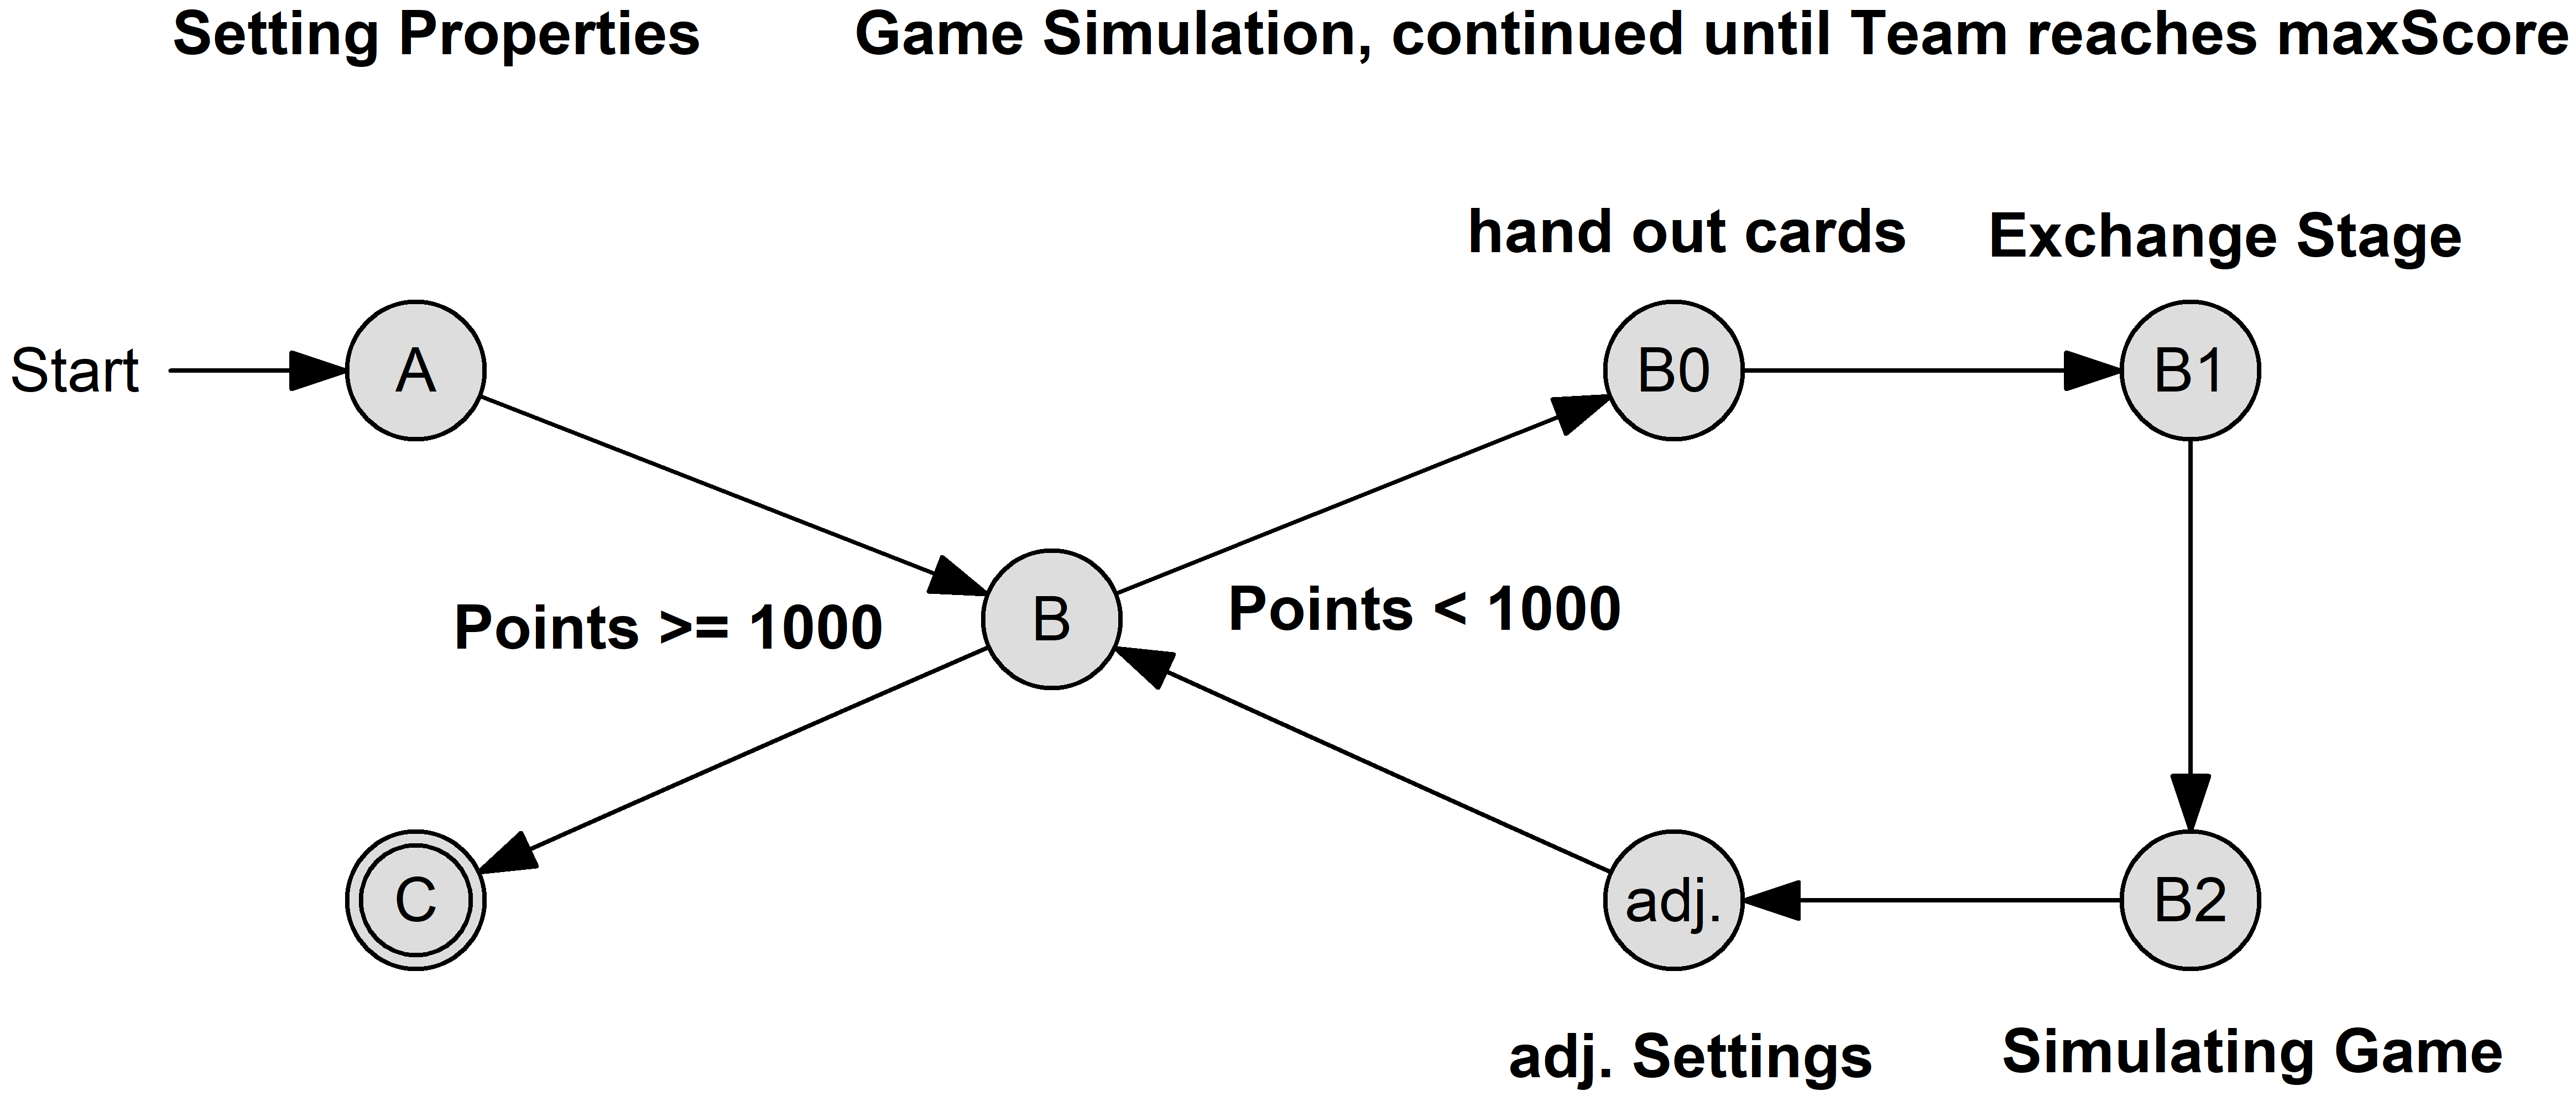
\includegraphics[width=0.5\textwidth]{Bilder/graph}
    \caption{Game model}
    \label{fig:meine-grafik}
\end{figure}

A game tree represents the different stages the game propagates through until one team reaches 1000 points and wins the game. This tree divides the game into sections that each deal with a game mechanism, each of which will be described in the following sections.

The game starts when four players divide into two teams and enter the game. These players each have assigned player behaviours $\alpha$ and are assigned a level of transparency of information $\beta$. The next subgame B is further divided into the distribution of cards (B.0), the exchange stage (B.1) and the active game of triumphing and laying cards (B.2). B.0 simulates the distribution of a card set to each player, each card set is represented by a value $X_i \in [0,1]$. The sum of all four card sets can be greater than 1, as the value of each set is not determined by single card values but rather their ability to be played in powerful combinations. This points distribution mechanism is a topic of discussion later in this essay again. The basic model only implements statistics in part B.0, however with the development of our model we will incorporate game theoretical aspects as well. The second part B.1 represents the Exchange Stage. Depending on a player’s cards and strategy, every player gives away three $\Delta X$ and receives three $\Delta X$, which can either be positive or negative. The payoff will be represented by a Util. In this section we will also define pass and receive functions to construct and define a Total Exchange Function semantically. The third part B.2 takes the card values X and the current score from part B.1 and processes these. They are used to determine the actual outcome of a game, reflecting the player’s strategies and accounting for possibilities to take higher risks due to score differences. This results in a Util  function that allocates the 100 available points per round and additional Tichu and double win points to the two teams.
In every round B, the dynamic or invariant parameters $\alpha, \beta, \gamma, \delta$ are considered. The repetition of subgame B ends when one team wins at 1000 points reached. Our first approximations consider $\beta$ and $\gamma$ as invariant.


\subsubsection{Subgame A}
To start a game of Tichu, we assign a player $\alpha_i$ and $\beta_i$ values. As assumed before, all $\beta_i$ are equal at either 0 or 1. This leaves two possibilities on $\beta$ and 16 possible combinations for $\alpha$. Due to the team aspects, symmetry and equal permutations reduce the number of combinations to six as seen below. We denote a combination as $\tilde{\alpha}_i$.\\
\begin{table}[h]
\resizebox{0.5\textwidth}{!}{%
\begin{tabular}{|c|c|c|}
\hline 
Player 1 $\backslash$ Player 2 & A & B \\ 
\hline 
A & 1 (AA) & 2 (AD = DA) \\ 
\hline 
B & 2 (DA = AD) & 3 (DD) \\
\hline 
\end{tabular}%
}
\end{table}
\begin{table}[h]
\resizebox{0.5\textwidth}{!}{%
\begin{tabular}{|c|l|l|l|}
\hline 
Player 1 $\backslash$ Player 2 & 1 & 2 & 3 \\ 
\hline 
1 & $\alpha_1$ (AAAA) & $\alpha_2$ (AAAD) & $\alpha_3$ (AADD) \\ 
\hline 
2 & $\alpha_2$ (ADAA) & $\alpha_4$ (ADAD) & $\alpha_5$ (DDAD) \\ 
\hline 
3 & $\alpha_3$ (DDAA) & $\alpha_5$ (ADDD) & $\alpha_6$ (DDDD) \\ 
\hline 
\end{tabular}%
} 
\end{table}
\subsection{Subgame B.0}
Our basic model considers B.0 as invariant under all $\alpha$, $\beta$, $\gamma$ and $\delta$. It is based on statistics gathered from collected online data and a survey we distributed. Initially we assign $X_i$ (a player’s distributed card set in each round) to be an element of the normal distribution with parameters $\mu, \sigma$. We set $\mu$ to 0.5 and define $X_i$ in the domain $1\geq X_i \geq 0$. We set $\sigma$ according to real world data and surveys. We have now ensured subgame B.0 always delivers an $X = \{X_1, …, X_4\}$, the card values used in the next two sections.


\subsection{Subgame B.1}
The aim of this section is to give a logical foundation for the Exchange Stage function we construct and show that it is indeed semantically viable. We shall first propose a few logical assumptions and define some key properties of a total exchange stage function before constructing a compilation of two simpler functions that pass and receive card values between players. First of all we definie some terms:
\begin{definition}["good" cards]
"Good" cards are for example bombs, high cards like ace or long, specific combinations that other players do not have.
\end{definition}
\begin{definition}["bad" cards]
Bad cards can rarely be played, for example deep cards or combinations that are never the highest combinations, so you rarely win a trick
\end{definition}
The following approximations were made to guide our definitions and constructions of functions:
\begin{enumerate}
\item A player can give “good” cards to his partner if and only if he has “good” cards.
\item A player can give “bad” cards to his opponents if and only if he has “bad” cards. 
\item The value of a card is subjective to a player. 
\item There is no absolute solution for every situation, the best solution is subjective to a player \\
\end{enumerate}
\begin{definition}[Player, Team, Partner and Opponent]
Given $\alpha$, $\beta$ and $X$, a player $P_i$ is called the triple ($\alpha_i$, $\beta_i$, $X_i$). 
On the set of players, we define an equivalence relation, where each class forms a Team $T_j$. Following conditions are true for players A ($\alpha_A$, $\beta_A$, $X_A$), B($\alpha_B$, $\beta_B$, $X_B$), C($\alpha_C$, $\beta_C$, $X_C$):
 \begin{axioms}[(P1)]
  \item A $\sim $ B (Reflexiv)
  \item A $\sim$ B $\Leftrightarrow$ B $\sim$ A (Symmetric)
  \item A $\sim$ B, B $\sim$ C $\Rightarrow$ A $\sim$ C (Transitivity)
  \end{axioms}
Players in the same Team will be called partners while players in another Team will be called opponents. We will write $PT_i$ for the Partner Team of $P_i$ and $OT_i$  for the Opponent Team of $P_i$.

We define $T_1 = [P_1,P_2]$  and $T_2 = [P_3,P_4]$. Therefore, $PT_1 = T_1$, $OT_1 = T_2$, $PT_2 = T_2$, $OT_2 = T_1$.

\end{definition}

\begin{definition}[Symmetric game perspective]
We will say, two players $P_i$, $P_j$ with  $i \neq j$ share a symmetric game perspective if $P_i = P_j$, $PT_i = PT_j$, $OT_i = OT_j$, in words: They have the same cards and the teams are identically from their point of view. 
\end{definition}
\begin{definition}[Total Exchange-Function]
We assume we have given $\alpha$, $\beta$, X. A function $\pi: \{0,1\}^8 \times [0,1]^4 \to [0,1]^4, (\alpha, \beta, X) \mapsto (X’)$ will be called an Exchange-function to B.1  if it applies to the following rules:
\paragraph{Randomness and Average}
$\alpha$, $\beta$, X are fixed. Then there is $\Delta X \subset [0,1]^4$ with $X’ \in \Delta X$. We will write $\pi^* (\alpha, \beta, X) = X^* \in \Delta X$ for the average of $\pi(\alpha, \beta, X)$. $\pi^*$ is a well-defined function, while $\pi$ allows random values around $\pi^*$.
\paragraph{Continuous and monotony of X}
$\alpha$, $\beta$ and X are fixed. If we change X in only one value that $X_i$ becomes $\widehat{X_i}$, it applies to the following rules:
\begin{axioms}[(C1)]
\item $\forall \epsilon > 0, \exists \delta > 0$ with $| X_i - \widehat{X_i}| < \delta$ \\$\Rightarrow | \pi^*(X_i) - \pi^*(\widehat{X_i}) | < \epsilon $
\item $\widehat{X_i} \leq X_i \Rightarrow \pi^*(\widehat{X_i}) \leq \pi(X_i)$
\end{axioms}

\paragraph{Symmetric outcome}
If two players $P_i$, $P_j$ have a symmetric game perspective, $\pi^*(X_i) = \pi^*(X_j)$
\end{definition}

Based on our approximations of this subgame, we can now construct an Exchange Function. We can split this task into a pass function and a receive function which respectively describe how a player gives away and receives cards.

If we first examine the pass function, we notice the following:\\
\begin{axioms}[(F1)]
\item For Player $P_i$, only $\alpha$, $\beta_i$ and $X_i$ are relevant.
\item Player $P_i$ does not differ between Opponents. 
\item The Player $P_i’s$ strategy does not change his behaviour on Opponents. 
\item In fact, he only needs to know his strategy, who he selects cards for and if known, his partner’s strategy. 
\end{axioms}

We put these facts together in a Diagram (the numbers represent diffrent exchange functions and $P_P$ - is a Player passing; $P_R$ - is a Player receiving):

\begin{table}[h]
\caption{Table 1.1} \bigskip
\label{tab:my-table}
\resizebox{0.5\textwidth}{!}{%
\begin{tabular}{l|l|ll|l|ll|}
\cline{2-7}
                                          & \multicolumn{3}{l|}{$\beta_i = 0$} & \multicolumn{3}{l|}{$\beta_i=1$} \\ \hline
\multicolumn{1}{|l|}{\multirow{3}{*}{OT}} & $P_R \backslash P_P$           & A         & D         &           & A         & D        \\ \cline{2-7} 
\multicolumn{1}{|l|}{}                    & A          & 1         & 1         & A         & 2         & 2        \\
\multicolumn{1}{|l|}{}                    & D          & 1         & 1         & D         & 2         & 2        \\ \hline
\multicolumn{1}{|l|}{\multirow{3}{*}{PT}} & $P_R \backslash P_P$              & A         & D         &           & A         & D        \\ \cline{2-7} 
\multicolumn{1}{|l|}{}                    & A          & 3         & 4         & A         & 5         & 6        \\
\multicolumn{1}{|l|}{}                    & D          & 3         & 4         & D         & 7         & 8        \\ \hline
\end{tabular}%
}
\end{table}
\paragraph{1.}
The Player is exchanging with an unknown Opponent. Therefore he will select a “bad” card, independent of his own strategy
\paragraph{2.}
The Player knows his opponent’s behaviour. He will also give him a “bad” card. The only difference is, that he knows better how the player will react on the card. This will change how an opponent receives the card, but is equivalent to 1. 
\paragraph{3./4.}
The player gives cards to his partner depending on his strategy. He does not know the strategy of his partner.
\paragraph{5.-8.}
The player knows his own and his partner’s strategy. Therefore his results will be better and the card difference will change.

This information motivates the following two definitions of the pass and receive function. Then, they  are compiled into one total Exchange Stage function. 

\begin{definition}[Pass-Function]
A function $\xi_{ji} : \{0,1\}^5 \to [-1,1], (\alpha, \beta_i) \to \hat{\xi}_{ji}$ will be called a pass function, if it describes what $P_i$ gives to $P_j$ according to certain rules:
\paragraph{Randomness and Average}
$\alpha$, $\beta_i$ are fixed. Then there is $\Delta  \hat{\xi_{ji}} \subset [-1,1]$ with  $\hat{\xi_{ji}} \in \Delta  \hat{\xi_{ji}}$. We will write $\{xi_{ji}\}^* (\alpha, \beta_i) =  \hat{\xi_{ji}} \in \Delta  \hat{\xi_{ji}}$ for the average of $\xi(\alpha, \beta_i)$. $\xi_{ji}^*$ is a well-defined function, while $\xi$ allows random values around $\xi^*$.
\paragraph{Symmetric outcome}
If two players $P_i$, $P_j$ have a symmetric game perspective towards each other,  $\hat{\xi_{ji}}^* =  \hat{\xi_{ji}}^*$
\paragraph{Normative aspects}
$\sum_{j = 1}^4 \hat{\xi_{ji}} = 1$
\paragraph{Realistic passing}
$\hat{\xi_{ii}} >>  \hat{\xi_{ji}}$ with $ i \neq j $
\end{definition}
\begin{definition}[Receive-Function]
A function $\eta_{ji}: \{0,1\} \times [-1,1] \to [-1,1], (\beta_i,  \hat{\xi_{ji}}) \mapsto \hat{\eta_{ji}}$ will be
called a “Receive-Function”, if it describes how $P_j$ receives cards from $P_i$ according to certain rules:
\paragraph{Randomness and Average}
$\beta_i$, $\hat{\xi_{ji}}$ are fixed. Then there is $\Delta  \hat{\eta_{ji}} \subset [-1,1]$ with  $\hat{\eta_{ji}} \in \Delta  \hat{\eta_{ji}}$. We will write $\{\eta_{ji}\}^* (\beta_i, \hat{\xi_{ji}}) =  \hat{\eta_{ji}} \in \Delta  \hat{\eta_{ji}}$ for the average of $\eta(\beta_i, \hat{\xi_{ji}})$. $\eta_{ji}^*$ is a well-defined function, while $\eta$ allows random values around $\eta^*$.
\paragraph{Symmetric outcome}
If two players $P_i$, $P_j$ have a symmetric game perspective towards each other:  $\hat{\xi_{ji}}^* =  \hat{\xi_{ij}}^*$
\paragraph{Self passing}
$\eta_{ii}(\hat{\xi_{ii}}) = \hat{\xi_{ii}} $
\end{definition}
\begin{definition}[Exchange-Function]
A function $\lambda_{ji}: \{0,1\}^5 \to [-1,1], \lambda_{ji} = \eta_{ji} \circ \xi_{ji}$ with $\eta_{ji}$ a Receive-Function and $\xi_{ji}$ a Pass-Function with existing $\alpha$, $\beta_i$.
\end{definition}
\begin{remark}[Construction]
We will now construct a Total Exchange Function based on an Exchange Function $\lambda_{ji}$. We will define $\Lambda = (\lambda_{ji})$ as a quadratic matrix. 
The Total Exchange-Function will be $\Lambda: X \mapsto \Lambda X = X’$
We now have to prove that this construction fits the definition.
\begin{axioms}[(1)]
\item Randomness and Average: This is induced from the combination of $\xi_{ji}$ and $\eta_{ji}$ in every argument. Therefore we can find an $\Delta \Lambda$ and $\Lambda^* $ which lead to $\Delta X $ and 
$X^*$
\item $\Lambda^*$ is a linear function, therefore continuous and monotone
\item Symmetric outcome is induced from the combination of $\xi_{ji}$ and $\eta_{ji}$ in every argument as in 1
\end{axioms}
We have now created a matrix $\Lambda$ which describes the Exchange Stage. To complete the definitions, we will introduce $ \Pi : \{0,1\}^8 \to M(4 \times 4, \mathbb{R}), (\alpha, \beta) \mapsto \Lambda $
\end{remark}

\subsection{Subgame B.2}
We shall now explore the active game, i.e. the laying and trumping of cards. We will first define a few new terms and three basic functions, including a double win probability function as well as a tichu announcement and tichu win probability function. We will then simulate the theory of an entire game consisting of multiple rounds and establish the different possible cases that can occur throughout a round.

We further assume players are completely rational and do not harm their own chances. Concretely, we presuppose that no counter-tichu will be called on a teammate’s tichu announcement. At this stage we can therefore treat two teammates as simply one element.

As a reminder, teams are defined by combining the two player triples $P_1$, $P_2$ and $P_3$, $P_4$into one element $T_1 = \{P1,P2\}$ and $T_2 = \{P3,P4\}$.

We shall start by defining the relevant terms and functions needed for this discussion. Let S define the game score, given by $S = \{S_1, S_2\} \in \mathbb{Z}^2$ where $S_1$ and $S_2$ are the scores of $T_1$ and $T_2$ respectively.

\begin{definition}[Double Win Function]
For each team we define a double win function $D_i(T_1, T_2)$.
\begin{align*}
D_i: ({0,1}^5 \times [0,1])^4 \to [0,1] (T1,T2) \mapsto d_i
\end{align*}
\end{definition}
This function returns the probability of a double win of each team for a round. As teams are always aiming for this bonus through a double win, we describe this function as independent of the current score and probably more dependent on the team strategies and the value of the cards. Whether or not player strategies have any influence on this probability will be heuristically/ empirically determined in the realisation section of this essay.

Next, as scoring a Tichu requires both calling and winning a Tichu, we separate the Tichu scoring opportunity into a Tichu announcement and Tichu winning function. For each team we define a Tichu announcement function $C_i(T_i, S)$, where $T_i$ are the respective teams and S is the current score. 


\begin{definition}[Tichu Announcment Function]
For each team we define a Tichu announcement function $C_i(T_i, S)$, where $T_i$ are the respective teams and S is the current score:
\begin{align*}
C_i: ({0,1}^5 \times [0,1])^2 \times \Z^2 \to [0,1] (T_i,S) \mapsto c_i
\end{align*}
\end{definition}
This function returns the Tichu announcement probability of each team for a round. It depends on a host of different variables including the player and team strategies as well as the current score and score difference. Such a function allows us to, for example, represent a greater probability of calling a Tichu when the opposing team has a large score margin or is very close to 1000 points.


\begin{definition}[Tichu Win Function]
Finally, we define the Tichu winning function $W_i(X_1, X_2,X_3,X_4)$ for each team as follows.
\begin{align*}
W_i: [0,1]^4 &\to [0,1] \\(X_1,X_2,X_3,X_4) &\mapsto t_i
\end{align*}
\end{definition}
This function indicates the probability that a team wins their Tichu bet in a given round. This too, is independent of score and game strategies as both teams will always want to win the Tichu bet. Rather, it depends completely on the teams’ card values.

With the above functions we can now simulate the theory of an entire game consisting of multiple rounds and establish the different possible cases that can occur throughout a round. We shall first explain how we simulate the probability of one or multiple Tichu calls and the scoring of a double win. Next, we shall explain how we calculate points for a team and then explore the following possible scenarios case by case.

\begin{definition}[binary random varibale]

We initially want to define a helper function, namely a \textbf{binary random variable} $Z(x): [0,1] \to [0,1]$ as a random variable that takes the value 1 with probability $x$ and $0$ with probability $1-x$.

\end{definition}

\subsubsection{Course of the game}
At the beginning we determine, through two binary random variables $Z(c_1)$ and $Z(c_2)$, whether team 1 or 2 announces a Tichu $(Z(c_1) = 1$ or $Z(c_2) = 1)$. Similarly, a binary random variable $Z(d_1)$ determines whether team 1 makes a double victory $(Z(d_1) = 1)$ or not $(Z(d_1) = 0)$. If $Z(d_1) = 0$, another binary random variable $Z(d'_2)$ determines if team 2 makes a double victory $(Z(d'_2) = 1)$ or not $(Z(d'_2) = 0)$. $d'_2$ is given by $d'_2 =d_2\cdot\frac{1}{1-d_1}$ because this case is only determined in $1-d_1\cdot 100$ percent of the cases. If $Z(d_1) = 1$, then $Z(d_2)$ is automatically 0, since a double victory of one team strictly excludes a double victory of the other.

Here we make the first differentiation between cases depending on whether a double win is scored or not. This is because a double win immediately awards +200 points to the scoring team regardless of the points distribution during the round. If a double win is not achieved by either team the points distribution must be calculated.

In the case $Z(d_1) = 1 \lor Z(d_2) = 1$, i.e. a double victory has been achieved, the score of team $T_i$ for which $Z(d_i) = 1$ applies will be increased by 200 points $(S_i += 200)$. Furthermore, if $Z(c_i) = 1$, Team $T_i$ has won its announced Tichu and therefore gets another 100 points $(S_i += 100)$. However, if the opposing team $T_j (i != j)$ has announced Tichu $(Z(c_j) = 1)$, this team loses 100 points $(S_j -= 100)$ as the calling player was unable to exit the round first.

The alternative case, $Z(d_1) = 0 \land Z(d_2) = 0$, requires more theory as we must determine how many points each team scores during a round. We assume that the announcement of Tichus has no effect on the distribution of points, although the opposing team may, for example, prioritise exiting the round first over scoring maximum points through won card values. We argue any such shift by a Tichu announcement in any specific round would generally be balanced out over all rounds of the game. Thus, we must only determine the points scored through the distribution of won cards.

For this calculation, we introduce two normally distributed random variables $n_1$ and $n_2$ whose mean value and standard deviation are to be determined in the realisation section of this essay. The purpose of these random variables is to simulate the fluctuations in scores obtained every round by both teams throughout the game. This will be explained further in the next section. The scored points for a round are to be calculated as follows: Let $X_{tot} = \sum_{i=1}^{4} X_i$ be the total sum of card values in this round, then
\begin{align*}
    &\Delta S_1 = (X_1\cdot n_1 + X_2\cdot n_2)/ X_{tot} \cdot 125 - 25\\
    &\Delta S_2 = (X_3\cdot n_1 + X_4\cdot n_2)/ X_{tot} * 125 - 25\\
\end{align*}
represent the change in score for each team for a round, where $\Delta S_1$ and $\Delta S_2$ are rounded to the nearest multiple of 5. Thus the change in score is calculated as a percentage of the card values for a specific round. The correctional factors 125 and -25 as well as the rounding serve to adjust the point value to the frame of a Tichu round.

Compounded onto the above theory are the following three cases as they relate to possible Tichu scenarios, namely: none, one or both teams announcing a Tichu:

\begin{axioms}[(C1)]
\item   If no team announces a Tichu $(Z(c_1) = 0 \land Z(c_2) = 0)$, then the point changes are simply added to the score.
\begin{gather*}
S_1 += \Delta S_1 \qquad S_2 += \Delta S_2
\end{gather*}
\item If one of the teams announces a Tichu $(Z(c_1) = 1$ XOR $Z(c_2) = 1)$ then a binary random variable $Z(w_i)$ determines whether this team makes the announced tichu. Here $w_i$ is, as defined earlier, the team's win probability. If $Z(w_i) = 1$ then the change of points is
\begin{gather*}
S_i += \Delta S_i + 100 \qquad S_j += \Delta S_j
\end{gather*}
Where $S_j$ represents the score of the opposing team. If $Z(w_i) = 0$ for the announced Tichu, then 100 points are subtracted from $S_i$. Other than that, the scores are added up as in case 1.
\item Both teams have announced a Tichu $(Z(c_1) = 1 \land Z(c_2) = 1)$. Since we assume every player to be rational, we assume that one of the two Tichus is definitely made. Now the probability that team 1 will make the Tichu is $w'_1 = \frac{w_1}{w_1+w_2}$, while $w'_2 =\frac{w_2}{w_1+w_2} = 1- w'_1$ represents the probability for team 2. Again, with the help of a binary random variable $Z(w'_1)$, we determine whether team 1 $(Z(w'_1) = 1)$ or team 2 $(Z(w'_1) = 0)$ has made the Tichu. If $T_i$ makes the Tichu and $T_j$ is the opponent team, the score is:

\begin{gather*}
S_i += \Delta S_i + 100 \qquad S_j += \Delta S_j - 100
\end{gather*}
This completes a round of the game. Now the subgames $B.0,B.1,B.2$ are repeated until $S_1 > 1000$ or $S_2 > 1000$ applies. In the following flowchart the process of $B.2$ is visualized once again:
\end{axioms}
(Schaubild)
\section{Realisation}
We shall now concretely define some of the theoretical aspects of our model: we want to ‘realise’ our model. For this we establish multiple distributions of card values and determine some distribution curves for the $/Delta  X$ in card value the exchange stage results in for each player. A dataset of more than 13,000 player statistics collected from onlinetichu.com using a web scrapper will help us gain statistical insight into our normal game and exchange stage mechanisms. Meanwhile, a quantitive survey we distributed will help us gain insight into risk and behaviour we are trying to simulate in our models and how sensitive our models should be to different kinds of risk. We will treat initially $\alpha$ and $\beta$ as constant, but then vary $\alpha$ in the subgame B.1 section and discuss ways to vary beta as well at the end of this section. start with modeling a function for B.0.

\subsection{Subgame B.0}
In our basic approach we assume an average card hand to have a value of $X_i = 0.5$, as the data from tichuonline.com shows the win rate almost normally distributed around 0.5, with an assumed symmetric normal distribution. $X_i = 0$ represents no chance of winning the game and $X_i = 1$ is equal to a guaranteed win. The question that arises is: to what percentage do players receive good enough cards to win a Tichu. We are now left with an arbitrary choice, which card set values correspond to which card combinations. Given that a Great Tichu is only won in 2.21$\%$ of all games, we can set $P(X_i \geq 0.9) = 0.0221$: the share of winning a great Tichu in reference to all games. This gives us a sigma of 0.199. Similarly, a Tichu is only won in 8.53$\%$ of all games, equalling $X_i\geq 0.78$. This results in the plot below that shows the probability a player has to receive a card set with a certain value.

\begin{figure}[h]
    \centering
    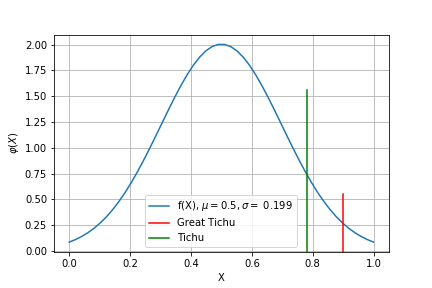
\includegraphics[width=0.5\textwidth]{Bilder/cards_distribution}
    \caption{cards distribution}
    \label{fig:meine-grafik}
    \centering
    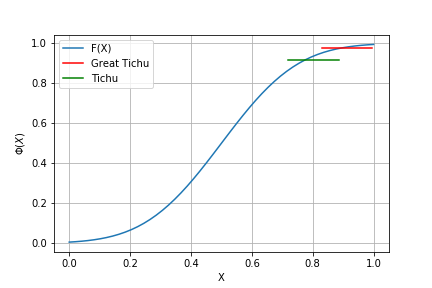
\includegraphics[width=0.5\textwidth]{Bilder/cards_distribution_cumultative}
    \caption{cards distribution cumultative}
    \label{fig:meine-grafik}
\end{figure}
We will always use this approximation and will not discuss it furthermore.

\subsubsection{Adjusting $\beta$}

If we set $\beta = 0$, we will only redefine the values, but the nash equilibrium will stay the same. Just from the cards, it is the best to play a mixed strategy for all cases. To enable this strategy in our simulation, we will now allow $\alpha$ to be in [0,1]. This will give us a well defined Exchange function as described before.

We always used $\beta$ as a fixed value in $\{0,1\}$. But in a real game, players can recognize the strategy of another player if they play enough games. Taking this into account, we will adjust $\beta$ during the game after each round. We decided to simulate the growth of knowledge with a logistic function, this is, in our point of view, the most realistic approximation of $\beta$ as at the beginning the growth of your information on other players is slowly but after some amount of games it speeded up. At the beginning, a Player has some information on the other players strategies (or does not). This value will be $\beta^{(0)}_{P}\in\{0,1\}$ for each Player $P\in\{1,2,3,4\}$. Note that now the knowledge of diffrent players $P_i\neq P_j$ can differ and develop throughout the game in diffrent ways based on the information given before the game. The player can get more information during the game. If he has much information, he will need more rounds to get new information on the other players. We will adjust this value to $\beta^{(1)}_{P}$ for the first round. This notation will lead us to the following adjusting, which will be described later on:
\begin{align*}
\beta^{(r+1)}_{P} = \frac{\beta^{(r)}_{P}
}{\beta^{(r)}_{P} + (1 - \beta^{(r)}_{P})} \cdot e^{-k}
\end{align*}
Where $k$ is in $\mathbb{R}_{>0}$ and $r$ is the number of rounds played. If $k$ is low, Players will learn slowly about other players strategies. If k is high, this process will be faster. We will now use $k = 0.2$, because we believe it is the most realistic function for $\beta$. An average round has <20 games and a knowledge of $80\%$ is way to high, while $10\%$ is low (see Chart):

\begin{figure}[h!]
    \centering
    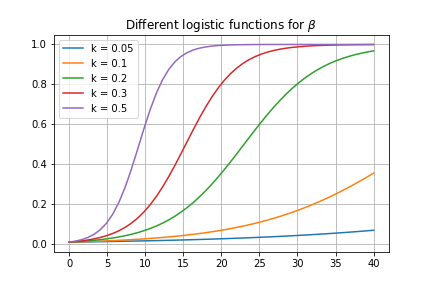
\includegraphics[width=0.5\textwidth]{Bilder/5_log}
    \caption{Adjusting $k$ for $\beta^{(r)}_{P}$}
    \label{fig:meine-grafik}
\end{figure}

\subsection{Subgame B.1}
The next game theoretical mechanism we want to realise is the exchange stage mechanism. We want to distinguish our models between passing to an opponent and passing to a partner and look at each of these types of trade individually. 

We start with the simplest model, namely passing exactly one card to any other player from their set of 14 cards. If he passes any random card, the average value of that card is $\frac{X_i}{14}$. This simple approximation is obviously not well-founded but we will expand on it shortly. There are two scenarios when passing a card to an opponent, one in which the player know the opponents behaviour and one in which there is no transparency of information. However, we treat the differences in the cases towards opponents as marginal and don’t consider these because a player will always want the worst result for an opponent, no matter the transparency of information. Therefore, there is only one possible exchange function towards an opponent. We call this function $\xi_O$ and assume it is normal distributed. We set $\mu = 0$, as normally giving away one card does not significantly change the value of your hand. According to this initial basic approach we set $2\sigma = \frac{1}{14}$, as it is the value of an average card and exchanging cards always includes the small possibility of building a new combination or bomb. The two graphs below describe this model.
 \\
\begin{figure}[h]
    \centering
    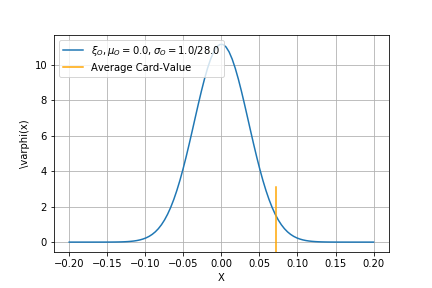
\includegraphics[width=0.5\textwidth]{Bilder/pass_function_ot}
    \caption{pass function for oppoenent player}
    \label{fig:meine-grafik}
    \centering
    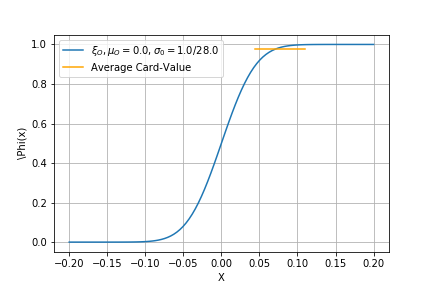
\includegraphics[width=0.5\textwidth]{Bilder/pass_function_ot_cumultative}
    \caption{pass function for the opponent player cumultative}
    \label{fig:meine-grafik}
\end{figure}
\\
The pass function towards a partner is more difficult but also more interesting to define. As well as aiming for an optimal result, partners can consider each others player behaviour and act on it if there exists transparency of information.

Again we assume the basic model from above, where the value of the average passed card is $X_i/14$ and normally distributed over a wide range. We therefore define $\xi_P$ as the Pass Function towards a Partner with $\mu_P =\frac{1}{14}$ and $\sigma_P = \frac{1}{14}$.


In addition to this simple model, partners have the possibility of taking advantage of each others known player types. If a player is defensive and requires above average cards to announce a Tichu he will more likely pass cards with higher value to his teammate. Correspondingly, if a player knows his partner is defensive, he can pass a lower valued card, while if a player knows his partner is aggressive, he would consider passing a high valued card. The following table shows what aggressive and defensive players pass with different amounts of information on their partner. \\
\begin{table}[h]
\caption{Table 2} \bigskip
\label{tab:my-table}
\resizebox{0.5\textwidth}{!}{%
\begin{tabular}{|l|ll|l|ll|}
\hline
\multicolumn{3}{|l|}{$\beta = 0$} & \multicolumn{3}{l|}{$\beta=1$} \\ \hline
\textit{$P_R \backslash P_P$}      & A       & D      & $P_R \backslash P_P$         & A        & D        \\ \hline
A              & -1      & +1     & A        & 0        & +2       \\
D              & -1      & +1     & D        & -2       & 0        \\ \hline
\end{tabular}%
}
\end{table}
We can construct a formula using this table: 
\begin{equation*}
z_{ji} = (1 - 2\cdot\alpha_i) + \beta_i \cdot (2\cdot\alpha_j - 1)
\end{equation*}

We will set $\mu = \mu_P + \frac{\sigma_P}{2} \cdot z_{ji}(\alpha, \beta)$. This will give us one function for $\xi_P$:

\begin{figure}[h]
    \centering
    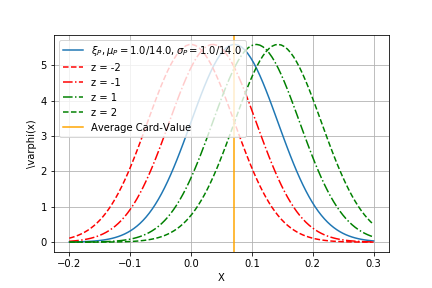
\includegraphics[width=0.5\textwidth]{Bilder/pass_function_p}
    \caption{pass function for your team partner}
    \label{fig:meine-grafik}
    \centering
    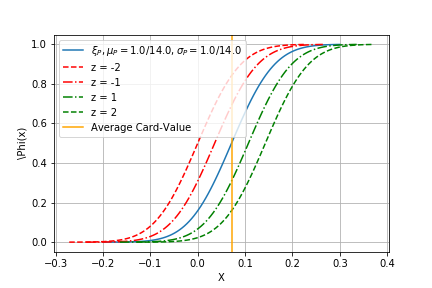
\includegraphics[width=0.5\textwidth]{Bilder/pass_function_p_cumultative}
    \caption{pass function for your teampartner cumultative}
    \label{fig:meine-grafik}
\end{figure}

A card which has a negative value to player $P_i$ can have a positive value to $P_j$ as this card could help build a new or stronger combination or bomb. Therefore, the card value can change during the exchange from $\hat{\xi}$ to $\hat{\eta}$. In this approach, we set $\eta_{ij} = id$, as the effect is very small in over a large number of games. 

We now have constructed Pass-functions $\xi_ji$ and a Receive Function $\eta_{ji} = 1$. We can use these functions to analyse the outcome of the Exchange-Stage $\lambda_{ji} = \xi_{ji}$. We can write $\Lambda$ using the average:

\begin{gather*}
\Lambda = \begin{pmatrix} 
1 - \xi_{21} & \xi_{12} & 0 & 0 \\
\xi_{21} & 1 - \xi_{12} & 0 & 0 \\
0 & 0 & 1 -  \xi_{43} & \xi_{34} \\
0 & 0 &  \xi_{43} & 1 - \xi_{34} \\
\end{pmatrix}
\end{gather*}

This can be further generalised. Now we no longer bet $\eta$ of the identity but let the card value and getting change. For the definition of the $\eta$ function we have made several basic assumptions. We assume that it also depends on the knowledge level of the players. For the $\eta$ function, we define a help function that represents a probability density. Basically, the $\eta$ function changes the value of the cards only slightly after they have been dealt, but there is a small probability that by getting the cards, the card value will improve. So here is the definition:
\begin{definition}[probability density]
The probability density $\rho$ is defined by a function which, normalized over the integral from -0.25 to $\infty$ 1, is called $\hat{\rho}$:
$$
\rho (t) := \frac{1}{4.39426613065366}\cdot\abs{\frac{\sin(4\cdot\pi\cdot t)}{t}}
$$
$$
\widehat{\rho} = \int\limits_{-0.25}^{\infty}\rho (t)\mathrm{d} t
$$
\end{definition}
\begin{figure}[h]
    \centering
    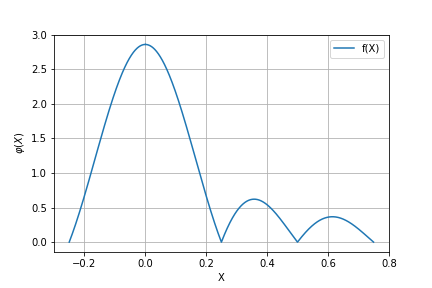
\includegraphics[width=0.5\textwidth]{Bilder/b1_e}
    \caption{$\rho$(t) - Wahrscheinlichkeitsdichte}
    \label{fig:meine-grafik}
    \centering
    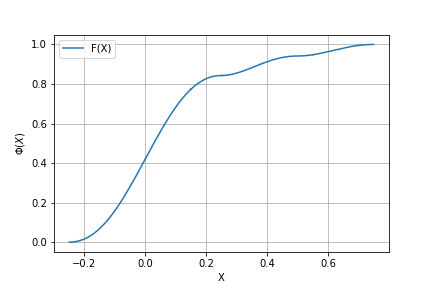
\includegraphics[width=0.5\textwidth]{Bilder/b1_f}
    \caption{$\widehat{\rho}(t) - Wahrscheinlichkeit$}
    \label{fig:meine-grafik}
\end{figure}
This probability value $\hat{\rho}(t)$ is then randomly generated for a $t\in [-0.25,0.7]$. This allows the $\eta$ function to be defined:
\begin{equation*}
\eta_{ij}(\xi_{ij}(X),\beta) = \xi_{ij}(X)\cdot(1+\mathrm{sgn}(X)\cdot\beta\cdot\langle\widehat{\rho}\rangle)
\end{equation*}
Furthermore set $\eta_{ij}(t)=0\;\forall t\not\in [-0.25, 0.75]$
So $\Lambda$ changes to:
\\ \\
\noindent\resizebox{0.45\textwidth}{!}{
$
\Lambda = \begin{pmatrix} 
1 - \sum\limits_{\substack{i=1 \\ i\neq 1}}^4\xi_{i1} & \eta_{21}(\xi_{21}) & \eta_{31}(\xi_{31}) & \eta_{41}(\xi_{41}) \\
\eta_{12}(\xi_{21}) & 1 - \sum\limits_{\substack{i=1 \\ i\neq 2}}^4\xi_{i2}  & \eta_{32}(\xi_{32}) & \eta_{42}(\xi_{42}) \\
\eta_{13}(\xi_{13}) & \eta_{23}(\xi_{23}) & 1 - \sum\limits_{\substack{i=1 \\ i\neq 3}}^4\xi_{i3}  & \eta_{43}(\xi_{43}) \\
\eta_{14}(\xi_{24}) & \eta_{23}(\xi_{23}) &  \eta_{34}(\xi_{43}) & 1 - \sum\limits_{\substack{i=1 \\ i\neq 4}}^4\xi_{i4} \\
\end{pmatrix}
$}

\subsection{Subgame B.2}
The last game mechanism we need to realise are the Tichu announcement and win functions that are separate from the functions that determine the value of and if they are theoretically good enough to make a Tichu. We factor in player behaviour and different types of risk that we have evaluated through a survey we distributed. After discussing and  implement the results of  this survey we further evaluate a graph from the earlier dataset showing Tichu announcement to tichu win probabilities. 

To approximate this problem as best as possible we have decided to look at the probability of announcing and winning a Tichu, rather than depending on and computing individual card sets. This is because we assume the average probabilities of winning a Tichu model the real game more realistically, over the course of many simulations, than assigning imaginary probabilities to each card. Following the assumptions made in earlier remarks in this essay we deny the possibility that 3 people announce a tichu and demand that one tichu must be won if 2 are announced. We can then assume that a team announces a tichu and any single player. We calculate the probabilities for announcing a Tichu through 2 factors:
\begin{enumerate}
\item Basic aggressiveness of the players (team$_{\alpha_1}$,team$_{\alpha_2}$)
\item  Additional risk tolerance depending on the score
\end{enumerate}
The basic aggressiveness of the players is converted to a basic aggressiveness of the team. This basic aggressiveness is derived from the player behaviour models. However, both aggressive and defensive players can take additional risk motivated through the current score of both teams. To assess the significance of these risks we conducted the following survey.

Respondents were asked about risk sensitiveness in three areas:
\begin{enumerate}[(1)]
\item diffrence in scores
\item edge of wedge
\item own distance to victory
\end{enumerate}
The scale here was the willingness to take risks from 1 to 10, whereby in category (1) and (2) 10 meant a lot of risk and 1 normal. For (3), 1 was normal risk and 10 was particularly low risk.
 As the survey revealed, Category (1) > Category (2) > Category (3) is in the ranking. The fluctuations in category (1) are 5 points.
 For category (2) 2.5 points and in (3) 0.5 points. In this weighting, these categories are also considered in the function.
The survey revealed the following data points (based on this point we generated with numpy a regression):
\paragraph{Cat.1}
$X=[0,100,200,300,400,500,600,700,800,900]$ \\ \\
$Y=[\frac{86}{21},\frac{83}{21},\frac{96}{21},\frac{114}{21},\frac{122}{21},\frac{142}{21},\frac{150}{21},\frac{170}{21},\frac{180}{21},\frac{183}{21}]$\\
\paragraph{Cat.2}\par
$X=[100,200,300,400,500,600,700,800]$ \\ \\
$Y=[\frac{140}{21},\frac{133}{21},\frac{111}{21},\frac{105}{21},\frac{100}{21},\frac{89}{21},\frac{88}{21},\frac{93}{21}]$\\
\paragraph{Cat.3}\par
$X=[100,200,300,400,500,600,700,800]$\\ \\
$Y=[\frac{94}{21},\frac{104}{21},\frac{105}{21},\frac{92}{21},\frac{105}{21},\frac{104}{21},\frac{92}{21},\frac{94}{21}]$
\begin{figure}[h]
    \centering
    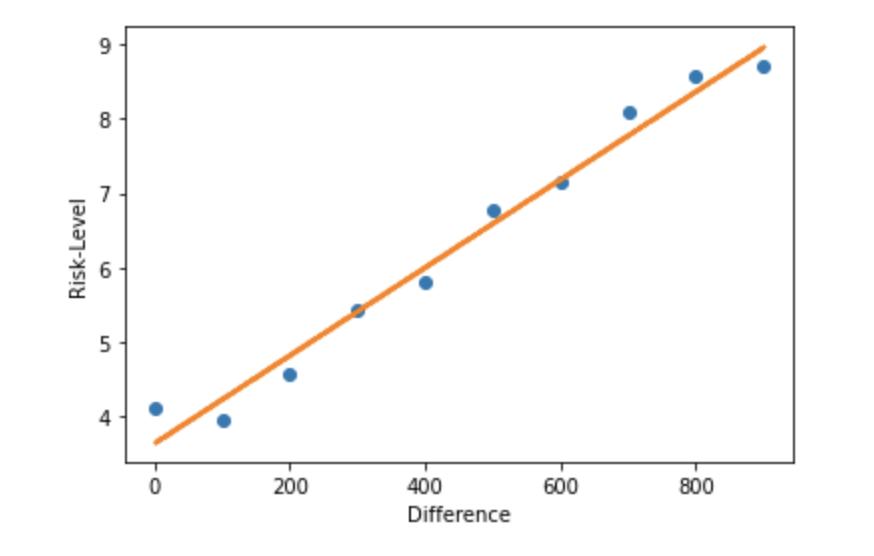
\includegraphics[width=0.5\textwidth]{Bilder/risk_level_diffrence_200steps}
    \caption{$f_1(x)=0.00591631\cdot x+3.65194805$}
    \label{fig:meine-grafik}
\end{figure}
\begin{figure}[h]
    \centering
    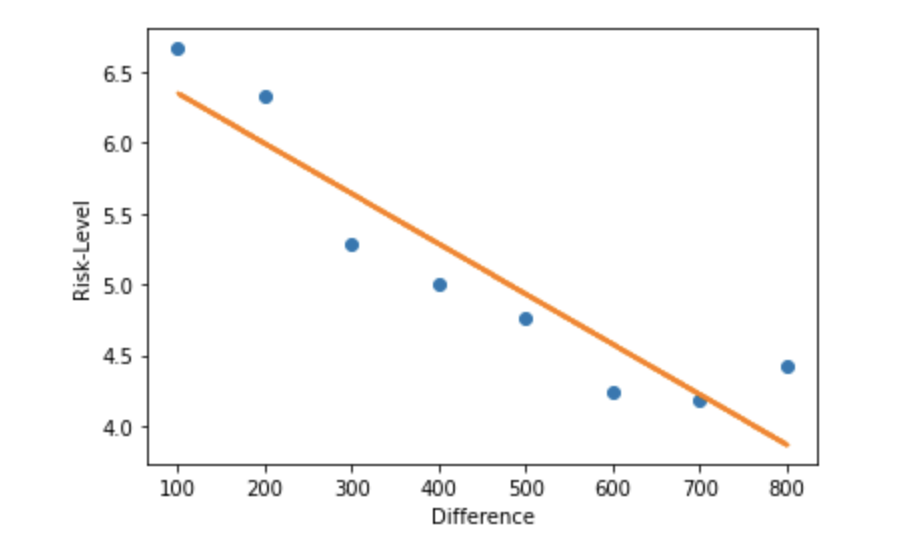
\includegraphics[width=0.5\textwidth]{Bilder/risk_level_diffrence_100steps}
    \caption{$f_2(x)=-0.00354308390\cdot x+6.70748299$}
    \label{fig:meine-grafik}
\end{figure}
\begin{figure}[h]
    \centering
    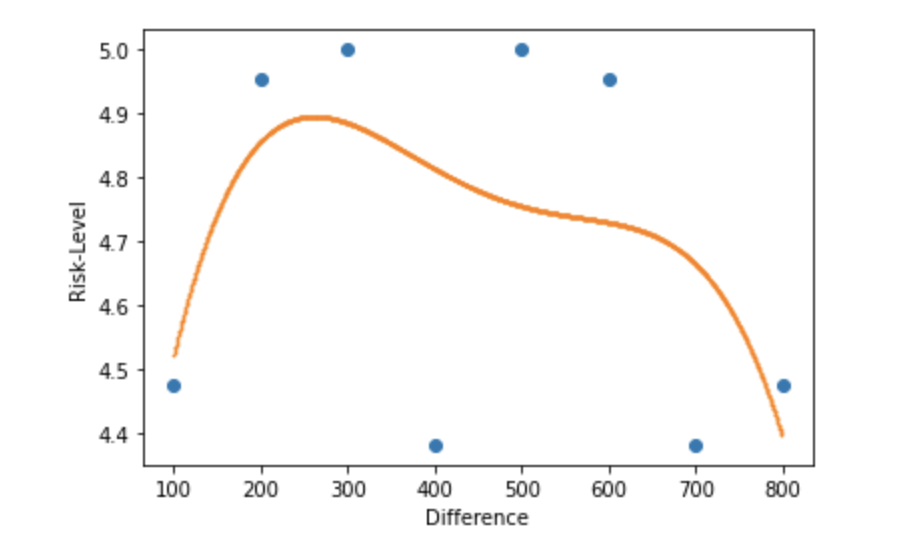
\includegraphics[width=0.5\textwidth]{Bilder/risk_level_diffrence_nonlinear}
    \caption{$f_3(x)=-3.87806638\cdot 10^{-11}\cdot x^4+7.31721982\cdot 10^{-8}\cdot x^3+ -4.95400433\cdot 10^{-5} \cdot x^2+ 1.36745860 \cdot 10^{-2} \cdot x+3.57993197$}
    \label{fig:meine-grafik}
\end{figure}
This increase should now be offset against the basic aggressiveness.
The following additional conditions are set:
If in category 1 the willingness to take risks is 8.5, the team should announce a 100$\%$ Tichu. With 4 it should have no effect.  In between it runs linear, as the function shows.
While category 1 can make a difference of up to 100$\%$, category 2 should have a maximum of 50$\%$. Again, linear.
Category 3 should bring in a maximum of 10$\%$. This function has level 4.
\begin{lstlisting}
f(play_1,play_2,t1,t2) :
    a=(play_1+play_2)/2
    if t2>=t1:
        d=(f1(t2-t1)-f1(0))/f1(900)
    else: 
        d=0
    if d>=1:
        return 1
    if t2<=200:
        b=0
    else:
        b=0.5*(f2(1000-t2)-f2(800))/
        (f2(100)-f2(800))
    if t1>=100 and t1<=800:
        c=0.1*(f3(1000-t1)-f3(800))/
        (f3(800)-f3(250))
    else:
        c=0
    if a+b-c+d>=1:
        return 1
    elif a+b-c+d>=0:
        return a+b-c+d
    else: return 0
\end{lstlisting}


In addition, there are other probabilities that must be known for the simulation. For example, the probability that a team will win the double or not. The average probability for the double victory is calculated from the average of all players: so total number of doubles divided by the total number of rounds. Also the probability that a player will win a Tichu must of course depend on the announcement frequency. This is what is described below.
So a graph of the tichu rate in relation to tichu announcements / rounds plots.
\begin{figure}[h]
    \centering
    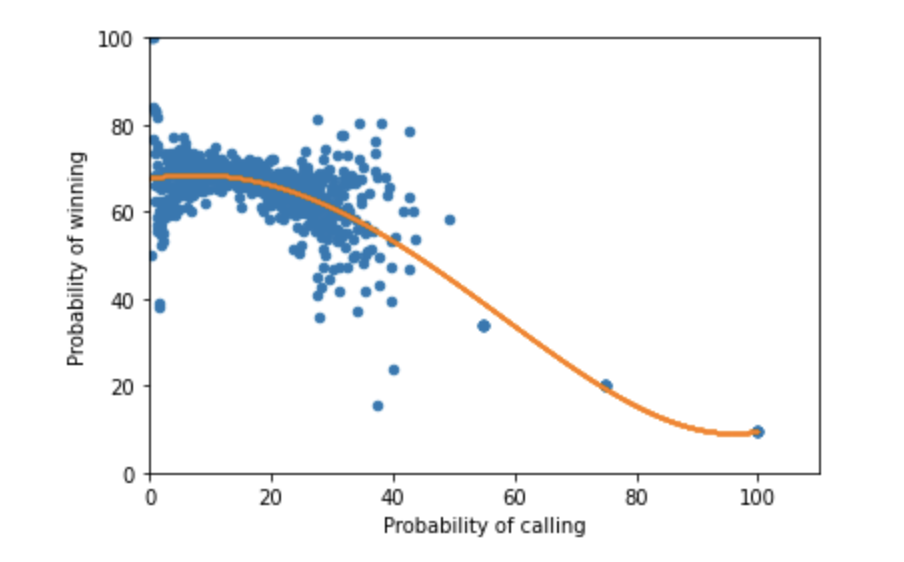
\includegraphics[width=0.5\textwidth]{Bilder/calling_winning_graph}
    \caption{$f4(x)=5.21140286\cdot 10^{-10}\cdot x^5+  7.51385614\cdot 10^{-07}\cdot x^4+  1.69471455\cdot 10^{-06}\cdot x^3+ -1.64932045\cdot 10^{-02}\cdot x^2+2.48230296\cdot 10^{-01}\cdot x + 67.7185027$}
    \label{fig:meine-grafik}
\end{figure}
The average probability for the double victory is calculated from the average of all players. So total number of doubles / total number of rounds.

From this data we have set up a function S, which assigns a probability to a player depending on his aggressiveness, with which he wins Tichus. The simulation of all these functions and the entire model is topic  of the next section.
\section{Simulation}
\subsubsection{Introduction to Software}
In order to simulate a Tichu according to our approximations, we have designed a python program consisting of three major files. We will give a brief introduction to these programs.

\paragraph{Python and Modules}
Our script is based on Python 3.7.1. and includes NumPy, SciPy and MatPlotLib as additional packages. 

\paragraph{Simulation}
This is the core of our program. We simulate a game with given start-values for alpha, beta, gamma and delta. In Addition, we set maxRounds and maxScore (40, 1000 by default). 
Due to the different approaches we made, we give different modes for each part of the simulation in a NumpyArray. The different parts of the Simulation are:
\begin{enumerate}
\item B0 – How do we generate the card values e.g. normal or linear distributed, equal
\item B1 – How do we exchange cards e.g. no exchange, average exchange, including receive
\item B2 – How do we distribute the points e.g. equal, normal distributed, highest, statistics
\item adj. $\alpha$ – Will $\alpha$ be adjusted after each round
\item adj. $\beta$ – Will $\beta$ be adjusted after each round e.g. increase
\item adj. $\gamma$ – How will the risk be adjusted e.g. according to surveys
\end{enumerate}
The used simulation modes are explained in our script on github-Link or trivial. 

\paragraph{Data Structure}
In order to save most of the data from a simulation, we created a class Solution which stores the data and a second class SimulationSet which can combine the data from many simulations. We also enabled saving and loading datasets and single simulations from files. Attention: We enabled pickle to load SolutionSet objects!  

\paragraph{Analysis and Plotting}
We created methods in the Solution-class to plot games and developments. To run and plot bigger simulations we used an external file which is also attached. 

\paragraph{Balancing and Switching}
Due to rounding errors in python, we observed that Team 2 wins more game than Team 1. 
To balance the game, we created a switching method, which switches the teams position every round. This leads to additional runtime but balances the game. 
We also created a method in the Solution class to switch the teams in the simulation. This is necessary to reduce the runtime. 

\subsection{Optimal strategy in "Exchange"-Stage}

First of all, we will have a look on the outcome of the Exchange Stage under different circumstances. But which outcome is the best for a team? We try to get a maximal value in three different ways:

\paragraph{Maximum}  We are only looking at the card value of the higher cards, because this can lead to a win of Tichu
\paragraph{Square Addition}  We sum the squares of both card values, because it doesn’t look only at the higher card value and consider both card values of the team.
\paragraph{Square Diffrence} We take the difference of the squares of both card values and try to minimize it, because it can be good to have balanced players. 
\\
\\
We try to find the nash equilibrium in all three cases and set $\beta = 0$. The players will not know which strategies the other players follow. We will only look at case $\beta = 0$ for case 1, because the information on his partners strategy will only create a bigger difference but will result in the same tactics. 

To determine the nash equilibrium, we will use the average values, including $\lambda_ji = 0$ for opponents. So we only look at the partner exchange with X = 0.5, $\mu = \frac{1}{14}$, $\sigma = \frac{1}{28}$.

We will show the average card values with $\beta =0$. The actual payoffs can differ:
\begin{table}[h]
\resizebox{0.5\textwidth}{!}{%
\begin{tabular}{|c|c|c|}
\hline 
Receiving $\backslash$ Passing & A & D \\ 
\hline 
A & 0.5, 0.5 & $0.5+\frac{1}{14}$, $0.5-\frac{1}{14}$\\ 
\hline 
D & $0.5-\frac{1}{14}$, $0.5+\frac{1}{14}$ & 0.5, 0.5 \\
\hline 
\end{tabular}%
}
\end{table}

1. Maximum:
\begin{table}[h]
\resizebox{0.5\textwidth}{!}{%
\begin{tabular}{|c|c|c|}
\hline 
Receiving $\backslash$ Passing & A & D \\ 
\hline 
A & 0.5, 0.5 & $0.5+\frac{1}{14}$, $0.5+\frac{1}{14}$\\ 
\hline 
D & $0.5+\frac{1}{14}$, $0.5+\frac{1}{14}$ & 0.5, 0.5 \\
\hline 
\end{tabular}%
}
\end{table}

2. Square Addition:
\begin{table}[h]
\resizebox{0.5\textwidth}{!}{%
\begin{tabular}{|c|c|c|}
\hline 
Receiving $\backslash$ Passing & A & D \\ 
\hline 
A & 0.5, 0.5 & $\frac{25}{49}$, $\frac{25}{49}$\\ 
\hline 
D & $\frac{25}{49}$, $\frac{25}{49}$ & 0.5, 0.5 \\
\hline 
\end{tabular}%
}
\end{table}

Assuming, Player 1 is playing strategy A with a probability of p, we will find the mixed nash-equilibrium p = 0.5, q = 0.5 if Player 2 is playing with a probability of q:

\begin{figure}[!ht]
    \centering
    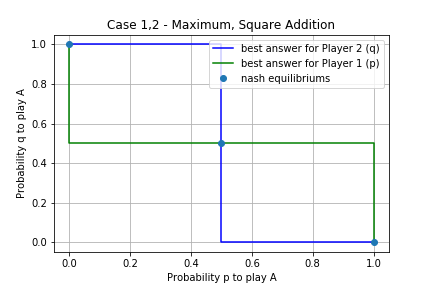
\includegraphics[width=0.5\textwidth]{Bilder/5_max}
    \caption{Case 1,2 - Maximum, Square Addition}
    \label{fig:meine-grafik}
\end{figure}

Anologously we can find the nash equilibrium for the third case.

3. Square Diffrence:

\resizebox{0.5\textwidth}{!}{%
\begin{tabular}{|c|c|c|}
\hline 
Receiving $\backslash$ Passing & A & D \\ 
\hline 
A & 0.0, 0.0 & $-\frac{1}{7}, \frac{1}{7}$ \\ 
\hline 
D & $-\frac{1}{7}, \frac{1}{7}$ & 0.0, 0.0 \\ 
\hline 
\end{tabular}%
}
\begin{figure}[!ht]
    \centering
    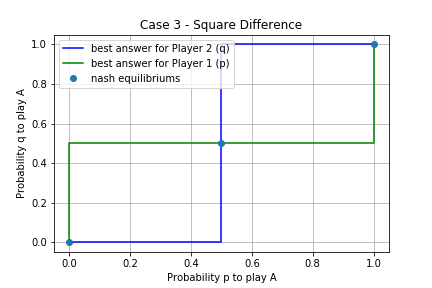
\includegraphics[width=0.5\textwidth]{Bilder/5_diff}
    \caption{Case 3 - Square Diffrence}
    \label{fig:meine-grafik}
\end{figure}
\subsection{Simulation of the game}
We have previously shown which strategy the other player should theoretically play, taking into account different metrics, if his opponent chooses a strategy and have hypothetically assumed average values (card values X=0.5) with the standard deviation we have determined.

We now try to generalize it and use the functions we developed in the theoretical part of the work. The goal of the game simulation is to simulate the course of a game depending on parameters given by us and thus to determine the best possible combination of $\alpha$ for the team.

The basis for each round is the card value X for each individual player. This is simulated by a normal distribution and is changed by the functions $\xi$ and $\eta$ during the exchange phase. The new card value X' is then saved and transferred for the game B.2, since the risk susceptibility is calculated from it.

In the 6 histograms below we show how phase B.0/B.1 works. As an example, 3 extreme cases are shown: 1. 1 game with 1000 points was played, where player 1 and 3 have $\alpha = 1$ and player 2 and 4 have $\alpha=0$. The $\beta$ was set to 1, since ideally one assumes omniscience. In the 2nd case the same was simulated for 10 games only. Finally in the 3rd case we left all parameters the same as in the 2nd case, only now we let the $\beta$ increase logistically during the game. In addition we plot there following graph (f(x)=93-x), which shows, if the teammate's aggressiveness is x, how high the own aggressiveness should reasonably be.
93$\%$is the value, which should result from the added aggressions, in order to achieve maximum points with the Tichu. The number 93 is the cumulative probability of the two team partners. It is the digit of the maximum of the function $x\cdot f(x)$, where f(x) is the probability of winning a tichu. Thus it gives the place of the maximum of the score.
At the edges the error of the theoretical model is of course bigger, because it is unrealistic that a player from the card distribution can get the tichu every round. 
Basically, the probability of the Tichu victory is maximized if both players announce with a probability of 46.5$\%$ and thus hit the maximum of the win, but at the same time the good cards of both players are used in the best possible way.

(Schaubilder)

The 3 cases show the influence of $\alpha$ on the card value and also on the exchange behaviour. It is noticeable in the range 0.8-1.0 that the aggressive players 1.3 improve the card value after the exchange phase and players 2.4 tend to worsen the card value.

We have now exemplarily seen how the parameters influence the card value, but the question arises, what is the optimal combination of player types, if you want to win the Tichu?

\subsubsection{Subgame B.2}
Of course the ideal situation would be to simulate every possible combination of our parameters a significant number of times to then get the best results. Due to our limited computation power we had to restrict our simulations. It was decided to simulate 100 games for each set of parameters. For the parameters we chose to fix $\alpha_3$ and $\alpha_4$ to $0.5$. And vary $\alpha_1$ and $\alpha_2$ from 0 to 1 in 0.01 increments. This means that team two plays with average aggressivity and team one’s aggressivity varies from totally passive to extremely aggressive. As in our simulation each player in a team is equal this allows us to use some symmetry, e.g. ($\alpha_1$,$\alpha_2$) = (1,0) yields the same result as (0,1). Therefore we could reduce the amount to simulate here. This left us with approximately 500.000 simulated games. Naturally this already is a tremendous task, especially considering our usage of python which is not the fastest.

For the Betas we therefore had to reduce the different cases as else this would have exploded into the uncomputable. Therefore we decided to select 3 cases:
\begin{enumerate}
\item $\beta$ equals zero for all players throughout every game. This is equal to no player knowing the strategies of the others
\item $\beta$ starts at zero but increases logistically throughout one game. Here the players deduce the strategies of the others as the game goes on
\item $\beta$ equals one throughout every game. Meaning all players not the other players strategies.
\end{enumerate}
Each of these simulations already took more than 16 hours. So doing varying beta more lies beyond our abilities. 

The graphs below show these results. The x-Axis represents the value of $\alpha_1$, the y-Axis the value for $\alpha_2$. Each dot represents 100 games played for these values of $\alpha_1$ and $\alpha_2$. The color represents the percentage of games won by team 1 for this configuration. Ranging from 40$\%$ or less (dark red) to 60$\%$ or more (dark blue). The left graph is Beta equal 0 for all players, the middle one for the logistical Beta and the right one for beta of 1.

As one can see an higher Beta makes the graph more blue, meaning that the more a team knows about the others the more likely it is to win with higher aggressivity. This is also what one would expect in a real game.
Consequently to get a better overview we only plotted the points where Team 1 won in more than 60$\%$ (first graphs) or lost in more than 60$\%$ (second graphs). Once again with the varying betas in the same order as above.

Here we can once again see that the more knowledge the players have the less extreme the difference between the teams gets. Moreover in the different colors we colored points that go roughly on a hyperbola branch (particularly visible in the left graph). Also one can see the trend of points converging to the two diagonals of the grid with higher betas.


For the better overview we have plotted all values in one graph, where you win  more than 60$\%$ of the games:

\begin{figure}[!ht]
    \centering
    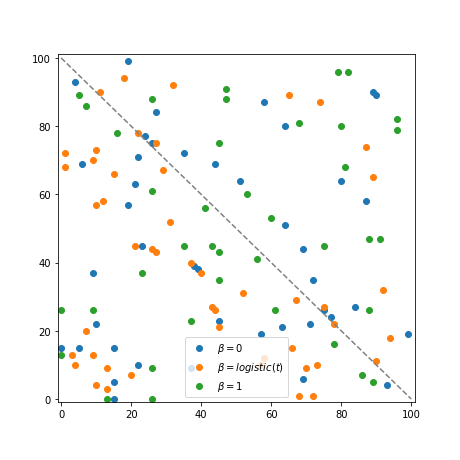
\includegraphics[width=0.35\textwidth]{Bilder/simulation_16}
    \caption{Case 3 - Square Diffrence}
    \label{fig:meine-grafik}
\end{figure}




\begin{figure*}[!ht]
	\centering
	\begin{subfigure}{0.3\textwidth}
	    \centering
	    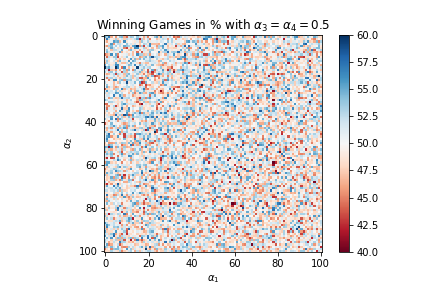
\includegraphics[width=1\linewidth]{Bilder/simulation_2_2}
	    \caption{Simulation 1}
	    \label{fig:meine-grafik}
    \end{subfigure}
	\begin{subfigure}{0.3\textwidth}
	    \centering
	    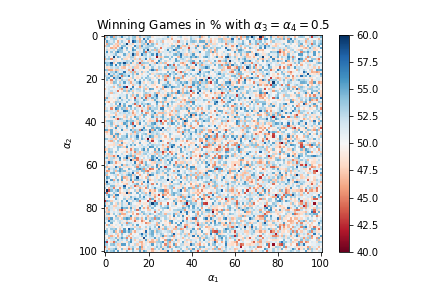
\includegraphics[width=1\linewidth]{Bilder/simulation_3_2}
	    \caption{Simulation 6}
	    \label{fig:meine-grafik}
    \end{subfigure}
	\begin{subfigure}{0.3\textwidth}
	    \centering
	    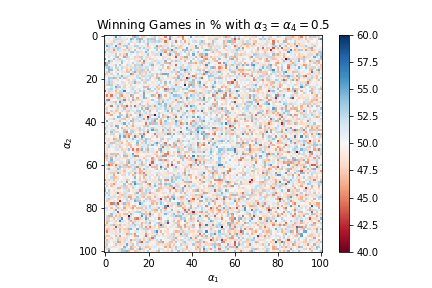
\includegraphics[width=1\linewidth]{Bilder/simulation_4_2}
	    \caption{Simulation 10}
	    \label{fig:meine-grafik}
	\end{subfigure}
\end{figure*}

\begin{figure*}[!ht]
	\centering
	\begin{subfigure}{.3\textwidth}
    	\centering
    	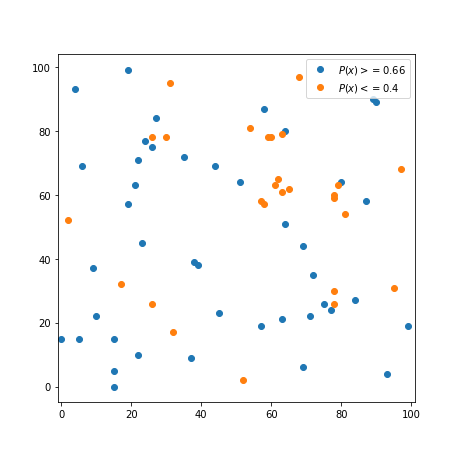
\includegraphics[width=1\linewidth]{Bilder/simulation_2_3}
    	\caption{Simulation 4}
    \label{fig:meine-grafik}
	\end{subfigure}%
		\begin{subfigure}{.3\textwidth}
	    \centering
	    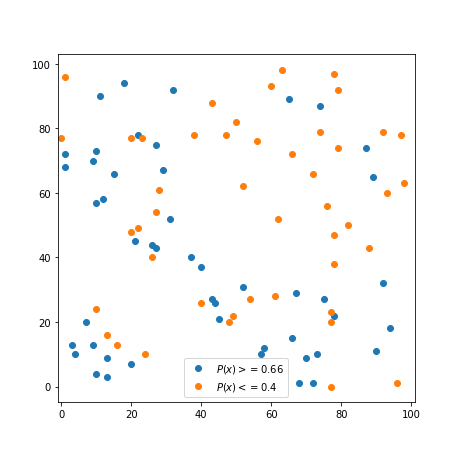
\includegraphics[width=1\linewidth]{Bilder/simulation_3_3}
	    \caption{Simulation 8}
	    \label{fig:meine-grafik}
    \end{subfigure}%
	\begin{subfigure}{.3\textwidth}
    	\centering
    	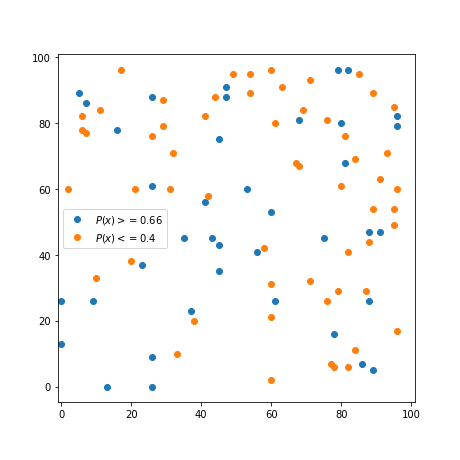
\includegraphics[width=1\linewidth]{Bilder/simulation_4_3}
    	\caption{Simulation 12}
    	\label{fig:meine-grafik}
	\end{subfigure}
\end{figure*}

\begin{figure*}[!ht]
	\centering
	\begin{subfigure}{.3\textwidth}%[!ht]
    	\centering
    	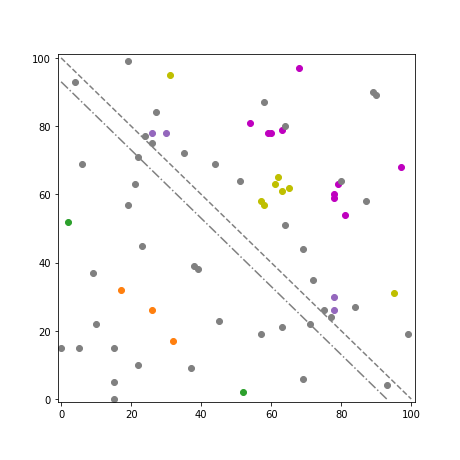
\includegraphics[width=1\linewidth]{Bilder/simulation_2_5}
    	\caption{Simulation Looses}
    	%\label{fig:meine-grafik}
	\end{subfigure}%
	\begin{subfigure}{.3\textwidth}%[!ht]
    	\centering
    	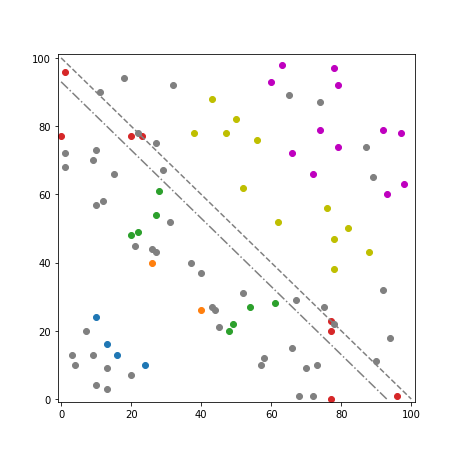
\includegraphics[width=1\linewidth]{Bilder/simulation_3_5}
    	\caption{Simulation Looses}
    	%\label{fig:meine-grafik}
    \end{subfigure}%
	\begin{subfigure}{.3\textwidth}%[!ht]
    	\centering
    	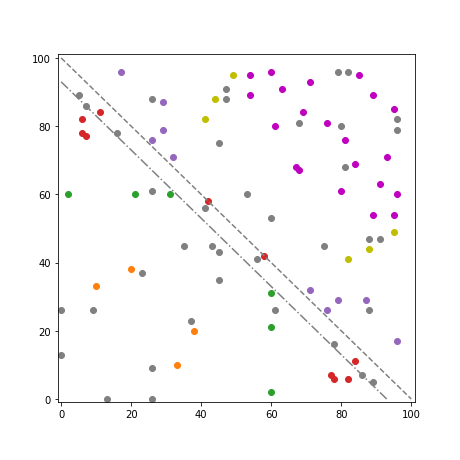
\includegraphics[width=1\linewidth]{Bilder/simulation_4_5}
    	\caption{Simulation Looses}
    	%\label{fig:meine-grafik}
	\end{subfigure}
\end{figure*}
\newpage

\section{Conclusion}
At this point we would like to discuss our errors and approximations in the model and explore further possibilities for improvement.

\subsubsection{Subgame B.0}
Here is probably the most essential approximation that the Great Tichu was neglected. This is of course essential for the scuffing, because it makes the scuffing much clearer. Each team partner (with Common Knowledge) would then give his team mate a very good card, because he himself can and needs no more Tichu. At the same time, the opponents will try to get the worst possible cards, like the dog that doesn't fit into any combination. Also the card 1 is usually nudged by the opponents in such a way that the player who has announced the Great Tichu comes second and thus must react to the request.
Problems could also result from normal distributions etc. Even if these were chosen sensibly, they do not always reflect reality very well. Calculating the values of cards based on their combination is extremely difficult, since the time course of the game also influences the value of a combination.

\subsubsection{Subgame B.1}

Basically this part has a very theoretical basis. There are of course more possibilities to change parameters and to cover different cases to get a better evaluation.
But even here, a certain arbitrariness is sometimes found in the eta and xi function, for example, but the result is meaningful, as can be seen at the Nash equilibrium. This could of course be further improved with certain calculations and statistical surveys.

\subsubsection{Subgame B.2}

The model has of course been simplified at one point or another.
First we start with the player model. It is of course very difficult to map a player type exactly. The division into 3 types is of course not small enough to reflect reality. Above all, the increase in risk will also depend on the type of player. Although the basic aggressiveness was taken as the underlying, the increase was calculated independently. But it is precisely the different situations that will provoke different human reactions. Even if the average of the survey showed this, it may be different for individuals.
Also the assumption of common knowledge will not apply to every player in every situation. For once we have also used this assumption to eradicate certain situations and not have to take them into account.
For example, we said that if a Tichu from Team 1 and Team 2 is announced, one of the two teams will win in any case. But it is also possible that a third player wins this Tichu and this without violating the assumption of common knowledge.
The irrational behaviour could occur for various reasons.
An example would be a player's lack of experience. After all, you cannot conclude with 100$\%$ certainty from your own cards that you are superior to your opponents.
The experience gained also goes hand in hand with certain strategies. For example, the convention that one shuffles an even card to the right and an odd card to the left. This is very useful, provided that both team members adhere to it. But it cannot be interpreted as Common Knowledge, because right even and left odd was chosen arbitrarily and would make sense as well, if it was swapped.
Another component that we have neglected is the timing of the game. By waiting for certain tricks, one can exclude that certain cards are still in the game and thus increase the probability for an own Tichu if necessary. However, this was not taken into account in this case.
One possible technical error is, for example, the interpolation of data from the onlinetichu.com website. Various errors can occur, especially during interpolation.


Especially since little or no data is provided for higher announcement rates, for example.
In the future, it would be possible to work on all these points in order to improve the model further.

\end{document}

